\documentclass[
  a4paper,
  abstract=on,
  captions=tableabove
  ]{scrartcl}

%section{Ignore warnings}

  \usepackage{silence}
  \WarningFilter{latex}{Marginpar on page}

%section{Packages}

  \usepackage{packages}
  
    % references
      \usepackage[
        style=authoryear,
        backend=biber,
        maxcitenames=3,
        maxbibnames=99,
        eprint=false,
        isbn=false
        ]{biblatex}

        % removes `p.` prefix
        \DeclareFieldFormat{postnote}{#1}
        \DeclareFieldFormat{multipostnote}{#1}

        % remove notes
        \AtEveryBibitem{\clearfield{note}}
        \AtEveryCitekey{\clearfield{note}}

      \addbibresource{references.bib}
  
  \usepackage{url}

  %subsection{extensions for the paper}

    \usepackage{siunitx}
    \sisetup{group-minimum-digits=4}

%section{New commands}

  \renewcommand{\hw}[1]{\textbf{#1}}

  \newcommand{\lsil}[1]{\lstinline[language=Python]{#1}}
  \newcommand{\mtrc}[1]{\textcolor{blue}{#1}}

  \newcommand{\sw}[1]{\texttt{#1}}

\begin{document}

%section{Title}

  \title{Social networks of lexical innovation}
  \subtitle{Investigating the diffusion of neologisms on Twitter}
  \author{Quirin Würschinger\\ LMU Munich}
  \maketitle

%section{Todos}

  % \listoftodos

%section{Abstract}
  \cleardoublepage

%section{floats}

  \listoffigures
  \listoftables

\cleardoublepage

%section{Abstract}

  \begin{abstract}

    Societies continually evolve and speakers coin and use new words to talk about innovative products and practices. While most lexical innovations fall into oblivion, others spread successfully and become part of the lexicon. This paper investigates the diffusion of 99 English neologisms on Twitter, from the start of the platform in 2006 until the end of 2018. Previous work on lexical innovation has almost exclusively relied on usage frequency counts for measuring diffusion. After applying several frequency-based measures to the dataset, I use social network analysis to study the sociolinguistic dynamics of diffusion in more detail, and I cross-evaluate the results obtained from both approaches.

    The results show that frequency counts lend themselves to approximate degrees of diffusion with varying success. While total usage frequency

    While usage frequency counts can be misleading, incorporating temporal dynamics of use provides a better picture of diffusion.

    However, frequency-based information alone fail to capture important sociolinguistic characteristics of diffusion. Social network information are shown to add valuable information about whether new words are known and used by an increasing number of individuals and communities of speakers.

    Firstly, I distinguish different pathways of diffusion depending on whether and to which degree new words show increasing vs. decreasing centralized use over time.
    Secondly, I show that social network information allow for a more fine-grained assessment of degrees of diffusion, for example when new words are used with increasing frequency when use their remains limited to certain parts of the speech community.
    Lastly, I compare the results based on usage frequency and on social network analysis. Besides notable discrepancies, we find a significant correlation between both types of information, which serves to cross-validate both approaches.

    The results suggest that social network information can complement frequency counts and that using information from both sources provides a more reliable and differentiated view of the sociolinguistic dynamics of diffusion.

    I argue that this is particularly important for investigating the diffusion of lexical innovations, as new words are often marked by high social indexicality and show substantial differences in use between communities of speakers. More generally, however, social network analysis shows great potential to study sociolinguistic dynamics of language variation and change beyond the domain of lexical innovation.

    \vspace{2\baselineskip}

    \textbf{Keywords}: lexicology, lexical innovation, sociolinguistics, diffusion, social media, Twitter, big data, social network analysis

  \end{abstract}

% text body

\section{Introduction}
  \label{sec:intro}

Societies continually evolve, new products and practices emerge, and speakers coin and adopt new words when they interact and share information. How do these new words spread in social networks of communicative interaction?

Covid-19 has recently spread through social contagion with shocking speed and has tragically affected the lives of people around the world. Its fatal consequences have demonstrated the devastating power of exponential diffusion in social networks. In a recent paper analysing contagion patterns of diseases in \emph{Nature Physics}, \textcite{Hebert-Dufresne2020MacroscopicPatterns} suggested that the spread of viruses follows principles of complex contagion through social reinforcement, and that it matches the dynamics of diffusion of cultural and linguistic innovations such as new words and internet memes. Does this confirm the widespread perception that new words \enquote{go viral}?

Influential sociolinguistic models of the spread of linguistic innovations like the S-curve model~\parencite{Milroy1992LinguisticVariation} share fundamental features with earlier economic models of diffusion~\parencite{Rogers1962DiffusionInnovations}, and such models show commonalities between the spread of cultural and linguistic innovations. It is often assumed that diffusion in social networks follows universal trajectories and that rates of spread depend on social dynamics such as network density and the presence or absence of weak ties~\parencite{Granovetter1977StrengthWeak}. Unlike research on biological and cultural diffusion processes, however, sociolinguistic research has only recently been provided with data sources that are equally suitable for large-scale, data-based approaches using social network analysis to study these phenomena empirically.

Social media platforms like Twitter have changed the way we communicate and how information spreads, and they offer large amounts of data for empirical research. Sociological research has been concerned with pressing issues regarding the impact of online social networks for the spread of hate speech, fake news and the power of \enquote{influencers}, bots and institutions on public opinions and elections, which increasingly strain the social fabric. For (socio-)linguists, social media provide large amounts of data of authentic language use which opens up new possibilities for the empirical study of language variation and change. The size of these datasets as well as their informal nature allow for large-scale studies on the use and spread of new words, for example, to gain insights about general trajectories~\parencite{Nini2017ApplicationGrowth} or about factors that influence whether new words spread successfully~\parencite{Grieve2018NaturalSelection}. Moreover, metadata about speakers allows studying aspects of diffusion that go beyond what can be captured by usage frequency alone. Recent work, for example, has used Twitter data to investigate the geographical spread of lexical innovations.~\parencite{Eisenstein2014DiffusionLexical,Grieve2017GeographicalPatterns,Grieve2018MappingLexical}

Data about the communicative interaction of speakers additionally allows performing network analyses of the social dynamics of diffusion processes. Network science approaches to social media data have been successfully employed in diverse fields, for example, to study the spread of diseases~\parencite{Lu2018AccurateInfluenza}, opinions~\parencite{West2014ExploitingSocial} and political attitudes~\parencite{PewResearchCenter2019NationalPolitics}. While the study of social networks has a long research tradition in sociolinguistics and has shaped influential models of diffusion~\parencite[e.g.][]{Milroy1985LinguisticChange}), large-scale network analyses of sociolinguistic phenomena have only recently become more widespread. These new data sources and methodological advances put computational sociolinguistics in an excellent position to gain new insights and to test long-standing theoretical models empirically.

In the area of lexical innovation, this can serve to evaluate important theoretical concepts like the role of early adopters, network density and weak ties \todo{references} in the diffusion of new words. For example, earlier approaches have used computational modelling to test the validity of the S-curve model~\parencite{Blythe2012ScurvesMechanisms}, and to model processes of simple and complex contagion of linguistic innovations in social networks~\parencite{Goel2016SocialDynamics}. Applying social network analysis to bigger samples of neologisms and tracking their diffusion on social media datasets promises to shed light on whether the adoption of new words remains limited to closely connected sub-communities or whether they reach larger parts of the speech community and whether individuals or groups drive this process.

This paper makes use of social media data and social network analysis to study the diffusion of lexical innovations on Twitter. Taking usage frequency as a baseline, we conduct a longitudinal study monitoring the use of a broad sample of neologisms to analyse their cumulated usage frequency as well as the temporal dynamics underlying their spread. We additionally use social network analyses of our neologism sample to get a better picture of the sociolinguistic dynamics at play, in order to assess different pathways and overall degrees of diffusion. Lastly, we compare both approaches to assess their validity, and we combine information from both sources to draw a more differentiated picture of diffusion.

The paper is structured as follows. Section 2 presents an overview of previous attempts to modelling and measuring the diffusion of lexical innovations in order to contextualise and define the present theoretical framework and its operationalisation for the empirical study. Section 3 provides information regarding the present sample of neologisms and the collection and composition of the Twitter dataset this study is based on. Section 4 describes the methodological procedure for analysing diffusion in this dataset, focusing on the construction and analysis of social networks. Section 5 presents the empirical results based on usage frequency and social network analysis, and from comparing both approaches to studying diffusion. Section 6 summarises and discusses these results and suggests theoretical implications and directions for future work.

\section{Modeling and measuring the diffusion of lexical innovations}

\section{Data}
  \label{sec:data}
  \subsection{Neologism sample}
    \label{subsec:neo-sample}

  I base my empirical study on a selection of 99 neologisms and study their use on Twitter from the start of the platform in 2006 to the end of 2018.

  The lexemes were selected to cover a broad spectrum of lexical innovation. Previous work by \textcite[115--147]{Kerremans2015WebNew} has identified four main clusters of neologisms on the conventionalization continuum: `non-conventionalization', `topicality or transitional conventionalization', `recurrent semi-conventionalization' and `advanced conventionalization`. My sample was designed to cover these categories and largely contains neologisms taken from the NeoCrawler, which uses dictionary-matching to retrieve a semi-automatic, bottom-up selection of recent neologisms on the web and on Twitter~\parencite{Kerremans2019UsingDatamining}. I have additionally included several lexemes that were statistically identified to have been increasing in frequency on Twitter in recent years by \textcite{Grieve2016AnalyzingLexical}.

  I limit my selection to neologisms whose diffusion started after 2006 to have full coverage of the incipient stages of their spread on Twitter.

  \subsection{Twitter data}
    \label{subsec:twitter-data}

    Twitter is a popular micro-blogging platform that was started in 2006 and has become one of the most popular social media platforms today.

    The Twitter community is not a perfect reflection of society and the speech community as a whole, of course, since certain social groups are over- or underrepresented according to social variables such as regional background and age.\todo{reference} Nevertheless, its broad user base and informal nature allow for a more representative picture of language use than domain-specific studies of, for example, newspaper corpora. Twitter corpora have been successfully used to identify patterns of sociolinguistic variation in numerous previous studies. A recent study by \textcite{Grieve2019MappingLexical} has, for example, shown the reliability of large-scale Twitter datasets for studying lexical variation.

    Twitter is particularly well-suited for studying lexical innovation due to the scale and types of data it provides, and due to the nature of language use on Twitter. The large size of Twitter's search index facilitates the quantitative study of neologisms, which requires large-scale datasets due to their inherently low frequency of occurrence. Twitter is widely used to discuss trends in society and technology, which makes it a good environment for studying the emergence of linguistic innovations. The informal and interactional nature of communication on Twitter fosters the rapid adoption of linguistic innovations, and the use of neologisms on social media platforms like Twitter often precedes and drives the diffusion of new words in more formal sources or on the web \parencite{Wurschinger2016UsingWeb}.

    \todo{retrospective, longitudinal, social network information, scope of the paper}
    % limited to Twitter, yet combination of frequency and SNA more robust

    The data for this study were collected using the Python library \emph{twint}, which emulates Twitter's Advanced Search Function. For each word in the sample, I performed a search query to retrospectively retrieve all tweets found in Twitter's search index. Due to the large volume of more frequent lexemes, I limited the sample to contain only candidates for which I could collect all entries found in Twitter's index. The combined dataset for all 99 lexemes in the sample contains 29,912,050 tweets. The first tweet dates from 5 May, 2006 and involves the neologism \ol{tweeter}, the last tweet in the collection is from 31 December, 2018, and includes \ol{dotard}.

\section{Method}
  \label{sec:method}

  I processed the dataset to remove duplicate tweets, tweets that do not contain tokens of the target neologism in the tweet text, and all instances where tokens only occurred as parts of usernames.\footnote{The post-processing as well as all quantitative analyses were performed in R~\parencite{RCoreTeam2018LanguageEnvironment}, and the source code is available on GitHub: \url{https://github.com/wuqui/sna}} Hashtag uses were included in the analysis. Retweets were excluded, since \emph{twint} does not consistently provide metadata which would allow to include retweeting activity in the social network analysis. The resulting dataset contains about 30 Mio. tweets which each contain at least one instance of the 99 neologism under investigation.

  To investigate the diffusion of these lexemes in terms of usage intensity \parencite{Stefanowitsch2017CorpusbasedPerspective}, I compared time-series data based on the neologisms' frequency of occurrence over time. I binned the number of tweets per lexeme in monthly intervals to weaken uninterpretable effects of daily fluctuations in use, and to achieve a reasonable resolution to compare the use of all lexemes, which differ regarding their overall lifespan. I visualize the resulting time series as presented in Figure XXX, adding the \emph{loess} function to indicate the smoothed trajectory of usage frequency over time.

  I calculated the coefficient of variance for all time series to capture different degrees of stability vs. volatility in the use of neologisms over time. The coefficient of variance~($c_{v}$) is a measure of the ratio of the standard deviation to the mean: $c_{v} = \frac{\sigma}{\mu}$. Higher values indicate higher degrees of variation in the use of a neologism, e.g. topical use of words such as \ol{burquini}; lower values indicate relatively stable use of words such as \ol{twitterverse}.

  To investigate the diffusion across social networks over time, I subset the time series into four time slices of equal size, relative to the total period of diffusion observed for each neologism. I set the starting point of diffusion to the first week in which there were more than two interactions which featured the target lexeme. This threshold was introduced to distinguish early, isolated ad-hoc uses of neologisms by single speakers from the start of accomodation processes during which new words increasingly spread in social networks of users on Twitter. This limit was validated empirically by testing different combinations of threshold values for the offset of number of users and interactions among early uses. Setting a low minimum level of interactions per week proved to reduce distortions in the size of time windows, and enabled a more robust coverage of the relevant periods of diffusion. For each neologism, I divided the time window from the start of its diffusion to the end of the period covered by the dataset into four equal time slices that are relative to the varying starting points of diffusion for all words in the sample. The starting points of each time slice are marked by dashed vertical lines in the usage frequency plots presented below (e.g. Figure XXX).

  To investigate the social dynamics of diffusion over time, I generated social networks graphs for each of these subsets. Nodes in the network represent speakers who have actively used the term in a tweet and speakers who have been involved in usage events in the form of a reply or a mention in interaction with others. The resulting graphs represent networks of communicative interaction. Communities are formed based on the dynamic communicative behaviour observed, rather than on information about users' social relations as found in follower--followee networks. This methodology is supported by previous research, which suggest that interactional networks of this kind are better indicators of social structure, since the dynamic communicative behaviour observed is more reliable and socially meaningful than static network information.~\parencite{Goel2016SocialDynamics, Huberman2008SocialNetworks} While users often follow thousands of accounts, their number of interactions with others provides a better picture of their individual social networks, which is much more limited in size~\parencite{Dunbar1992NeocortexSize}.

  To construct the networks, I extracted users and interactions from the dataset to build a directed graph.\footnote{I used several \emph{R} packages~\parencite{RCoreTeam2018LanguageEnvironment} from the \emph{tidyverse}~\parencite{Wickham2019WelcomeTidyverse} for the network pre-processing, \emph{igraph} and \emph{tidygraph} were used for constructing the networks and for calculating network metrics.} Nodes in the graph correspond to individual Twitter users, edges represent interactions between users. I capture multiple interactions between speakers by using edge weights, and I account for active vs. passive roles in interaction by using directed edges. I assessed the social diffusion of all neologisms quantitatively by generating and comparing several network metrics, and I produced network visualisations for all subsets for more detailed, qualitative analyses.

  On the graph level, I rely on the measures of \emph{degree centralization} and \emph{modularity} to quantify the degree of diffusion for each subset.

  Degree centralization~\parencite{Freeman1978CentralitySocial} is a graph-level measure for the distribution of node centralities in a graph. Nodes have high centrality scores when they are involved in many interactions in the network and thus play a `central' role in the social graph of users. The degree centrality of a graph indicates the extent of the variation of degree centalities of nodes in the graph. A graph is highly centralized when the connections of nodes in the network are skewed, so that they center around one or few individual nodes. In the context of diffusion, the graph of a neologism would have high centralization in early stages, for example, when its use is largely confined to one or few centralized clusters of speakers. Diffusion leads to decreasing centralization when use of the term extends to new speakers and communities and the distribution of interactions in the speech community shows greater dispersion.

  The normalized degree centralization of a graph is calculated by dividing its centrality score by the maximum theoretical score for a graph with the same number of nodes.\todo{insert formula} This enables the comparison of graphs of different sizes, which is essential for drawing comparisons across lexems in the present context. The neologisms under investigation differ with regard to their lifespan and usage intensity, which results in substantial quantitative differences in network size. This needs to be controlled for to allow for an investigation of structural differences of the communities involved in their use.

  Modularity~\parencite{Blondel2008FastUnfolding} is a popular measure for detecting the community structure of graphs. It is commonly used to identify clusters in a network and provides an overall measure for the strength of division of a network into modules. In the social context, this corresponds to the extent to which the social network of a community is fragmented into sub-communities. Networks with high modularity are characterized by dense connections within sub-communities, but sparse connections across sub-communities. In the context of the spread of new words on Twitter, diffusion leads from use limited to one or few densely connected communities to use in more and more independent communities. This is reflected by higher degrees of modularity of the full graph representing the speech community as a whole. Modularity complements degree centralization since it provides additional information about the number and size of sub-communities who use the target words. I rely on the modularity algorithm to perform community detection, and I visualize the 8 biggest subcommunties in each graph by color.

  Since modularity is sensitive to the number of edges and nodes in a graph, and thus cannot provide reliable results for comparing graphs of different size, I use degree centralization to analyse diffusion over time, and to assess differences in degrees of diffusion between lexemes on the macro-level. Its conceptual clarity and reliable normalization allow for more robust comparisons on the macro-level.

  For visualizing network graphs, I rely on the Force Atlas 2 algorithm~\parencite{Jacomy2014ForceAtlas2Continuous} as implemented in \emph{Gephi}~\parencite{Bastian2009GephiOpen}. Attempts to evaluate and compare these visualisations with results obtained from different algorithms such as Multi-Dimensional Scaling and Kamada Kawai showed similar results across methods for parts of the dataset, but could not be used for the full dataset due to the computational complexity involved in the generation of large-size graphs of high-frequency neologism. Force Atlas 2 is particularly well-suited for handling social networks in big data contexts and has been widely applied in network science approaches to Twitter data~ \parencite{Bruns2012HowLong,Gerlitz2013MiningOne,Bliss2012TwitterReciprocal}. To assess and visualize the influence of individual users in the social network, I use the PageRank algorithm~\parencite{Brin1998AnatomyLargeScale} (visualized by node size), and I account for varying degrees of strength in the connection between users by using edge weigths for repeated interactions (visualized by edge thickness).

\section{Results}
  \label{sec:results}

  \subsection{Usage frequency and diffusion}
    \label{subsec:freq}

    \subsubsection{Total usage frequency}
      \label{subsec:total-freq}

      As described in Section~XXX, successful diffusion involves an increase in the number of speakers and communities who know and use a new word. The degree of diffusion of new words is often approximated by usage frequency, i.e. by how many times speakers have used these words in the corpus. The most fundamental way of using this information is to cumulate usage counts and to rely on the total number of uses observed. The underlying assumption is that neologisms that have been used very frequently in the corpus are likely to be familiar to a large group of speakers who have actively produced the observed uses (\enquote{corpus-as-output}) or have been passively exposed to these neologisms (\enquote{corpus-as-input}).~\parencite{Stefanowitsch2017CorpusbasedPerspective} Aggregating all instances of usage to total counts is taken to represent the total amount of exposure or active usage, indicating the degree of conventionality in the speech community. In the following, I will use this most basic measure of diffusion as a baseline before I zoom in to get a more differentiated picture of the temporal and social dynamics of diffusion.

      The present sample of neologisms covers a broad spectrum of usage frequency. Table~\ref{tab:freq-total} presents the candidates under investigation in four groups: six examples around the minimum, around the median, and around the maximum total usage frequency observed in the corpus, as well as six words that will serve as case studies in the following sections. These cases reflect a diverse set of prototypical examples of diffusion patterns, and I will use these cases to illustrate more detailed characteristics of diffusion before I present the general patterns found for the full sample of neologisms.

      \begin{table}
        \caption[Total use frequency counts]{Total usage frequency (\textsc{freq}) in the corpus.}
        \label{tab:freq-total}
        \centering
        \begin{subtable}{.4\linewidth}
          \subcaption{Most frequent lexemes.}
          \label{subtab:freq-total-max}
          \centering
          \begin{tabular}{l S[table-format=7]}
            \toprule
            Lexeme       & {\textsc{freq}}  \\
            \midrule
            tweeter      & 7367174 \\
            fleek        & 3412807 \\
            bromance     & 2662767 \\
            twitterverse & 1486873 \\
            blockchain   & 1444300 \\
            smartwatch   & 1106906 \\
            \bottomrule
          \end{tabular}
        \end{subtable}
        \begin{subtable}{.4\linewidth}
          \subcaption{Examples around the median.}
          \label{subtab:freq-total-median}
          \centering
          \begin{tabular}{l S[table-format=5]}
            \toprule
            Lexeme               & {\textsc{freq}} \\
            \midrule
            white fragility      & 26688  \\
            monthiversary        & 23607  \\
            helicopter parenting & 26393  \\
            deepfake             & 20101  \\
            newsjacking          & 20930  \\
            twittosphere         & 20035  \\
            \bottomrule
          \end{tabular}
        \end{subtable}

      \vspace{\baselineskip}

        \begin{subtable}{.4\linewidth}
          \subcaption{Least frequent lexemes.}
          \label{subtab:freq-total-min}
          \centering
          \begin{tabular}{l S[table-format=3]}
            \toprule
            Lexeme     & {\textsc{freq}} \\
            \midrule
            microflat  & 426             \\
            dogfishing & 399             \\
            begpacker  & 283             \\
            halfalogue & 245             \\
            rapugee    & 182             \\
            bediquette & 164             \\
            \bottomrule
          \end{tabular}
        \end{subtable}
        \begin{subtable}{.4\linewidth}
          \subcaption{Case study selection.}
          \label{subtab:freq-total-cases}
          \centering
          \begin{tabular}{l S[table-format=7]}
            \toprule
            Lexeme       & {\textsc{freq}}  \\
            \midrule
            alt-right    & 1012150 \\
            solopreneur  & 282026  \\
            hyperlocal   & 209937  \\
            alt-left     & 167124  \\
            upskill      & 57941   \\
            poppygate    & 3807    \\
            \bottomrule
          \end{tabular}
        \end{subtable}
      \end{table}

      The clustering of neologisms on the basis of their total usage frequency presented in Table~\ref{tab:freq-total} largely seems to fit intuitions about diverging degrees of conventionality between the frequency-based groups \ref{subtab:freq-total-max}, \ref{subtab:freq-total-median}, and \ref{subtab:freq-total-min}. Neologisms such as \ol{blockchain} and \ol{smartwatch}, which are probably familiar to most readers, can be assumed to be more conventional than neologisms from the other end of the frequency continuum such as \ol{dogfishing} (\enquote{using a dog to get a date}) or \ol{begpacker} (\enquote{backpackers funding their holidays by begging}).

      However, total frequency counts only provide a limited picture of diffusion since they are insensitive to temporal dynamics of usage, Neglecting temporal information about the lifespan and the period of active use of a new word can distort the quantitave assessment of its degree of conventionality in two directions. Firstly, it bears the danger of overestimating the status of words such as \ol{millenium bug}\footnote{The neologisms \ol{millenium bug} was used to refer to ancipated technical problems caused by inconsistent formatting of timestamps at the turn of the century.}, whose total usage frequency largely goes back to a short period of highly intensive usage, after which they fall into oblivion and are unfamiliar to following generations of speakers, and eventually become obsolete. Secondly, total counts can underestimate the conventionality of words such as \ol{coronavirus}, which have already become familiar to the vast majority of speakers, but show comparatively moderate total frequency counts, since they have started to diffuse only fairly recently.

      Among the most frequent neologisms presented in Table~\ref{subtab:freq-total-max}, words such as \ol{twitterverse} and \ol{blockchain}, for example, have similar total frequency counts, but differ significantly with regard to their temporal usage profiles. The neologism \ol{twitterverse} has been in use ever since the start of Twitter, while the diffusion of the much younger \ol{blockchain} only started in 2012. Due to its shorter lifespan, \ol{blockchain} accumulated roughly the same number of uses, but shows significantly higher usage intensity in the more recent past, and could be assumed to be familiar to bigger parts of the speech community.

  \marginpar{total usage frequency will be used to evaluate the social network metrics}

      Similar effects are even more pronounced in the remaining groups of neologisms, since words from the lower ranges of the frequency spectrum are typically affected more strongly by temporal variation in their use. In the following sections, I will include temporal information to provide a more fine-grained picture of diffusion.


    \subsubsection{Cumulative frequency}

      \marginpar{trend: convex vs. concave}

      Visualising the cumulative increase in usage frequency of new words complements total counts by taking into account the temporal dynamics of their usage intensity over time. Figure~\ref{fig:freq_cum_cases} presents this information for the case study selection.

      \begin{figure}
        \caption[Cumulative increase in usage frequency]{Cumulative increase in usage frequency for case studies.\protect\footnotemark}
        \label{fig:freq_cum_cases}
        \centering
        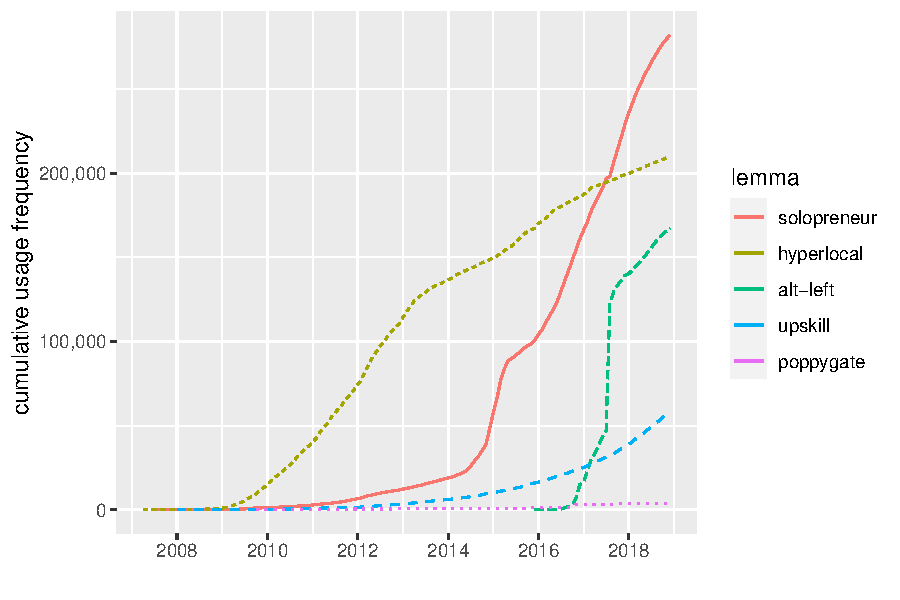
\includegraphics[width=.8\linewidth]{img/freq_cum_cases.pdf}
      \end{figure}
      \footnotetext{\ol{alt-right} was omitted from this plot because its high usage frequency would have inhibited the interpretability of the other lexemes; its frequency over time is presented in Figure \ref{subfig:freq_temp_alt-right}.}

      While the end points of the trajectories in Figure~\ref{fig:freq_cum_cases} mark the target words' total frequency counts as shown in Table~\ref{subtab:freq-total-cases}, the offsets and slopes of the trajectories of usage frequency reveal additional characteristics about differences in their diffusion patterns.

      The selected neologisms differ regarding their total lifespan observed, which is indicated by diverging starting points of diffusion. The term \ol{hyperlocal}, for example, is the oldest new word among the selected neologisms, and it is commonly used to refer to information that has a strong focus on local facts and events. While it was hardly used in the first years of Twitter, it started to increase in its use in 2009, and it was added to the OED's Third Edition in 2015. Around this time, the neologism \ol{solopreneur} only started to significantly increase in its use. A blend of \ol{solo} and \ol{entrepeneur}, it keeps a low, flat trajectory of sporadic use for about 7 years after its first appearance in the corpus. The first two attestations in the corpus indicate the sense of novelty and scepticism towards the term in its early phases:

      \renewcommand{\labelenumi}{(\arabic{enumi})}
      \begin{enumerate}
        \item I'm trying to figure out if I like the term \enquote{solopreneur} I just read. (27 July, 2007)
        \item hmmmmmmm new word added to my vocab = \enquote{solopreneur} !! (6 January, 2008)
      \end{enumerate}

      Most speakers increasingly \enquote{like the term} and \enquote{add them to their vocabulary} only much later, after 2014, when the phenomenon of individual entrepreneurship attracts increasing conceptual salience in the community, which seems to be both reflected and propagated by the publication of several self-help books for entrepreneurs in this year, which all explicitly use this new term in their titles (e.g. the popular guide \emph{Free Tools for Writers, Bloggers and Solopreneurs} by Karen Banes). The following short, but intense period of use results in a higher overall number of uses for \ol{solopreneur} as compared with \ol{hyperlocal}, even though the use of the latter term shows a longer lifespan of continual use.

      In addition to lifespan differences, the slopes of the cumulative trajectories in Figure~\ref{fig:freq_cum_cases} indicate differences regarding the dynamics of diffusion underlying the aggregated total number of uses over time.

      Neologisms such as \ol{hyperlocal} and \ol{upskill} (\enquote{to learn new skills}) show a steady, gradual increase in usage frequency over longer periods of time. By contrast, the use of other candidates such as \ol{solopreneur} and \ol{alt-left} is much less stable and evenly distributed over time.

      In the case of \ol{solopreneur}, we observe a big spike in frequency following its increased popularity in the entrepreneurial community in 2014. While it shows the highest total frequency count in Figure~\ref{fig:freq_cum_cases}, the majority of its uses fall into the second part of its observed lifespan.

      An even shorter and steeper increase can be seen in the use of \ol{alt-left}, which is the youngest neologism to enter the scene at the end of 2015. \ol{alt-left} was coined as a counterpart to the term \ol{alt-right}. The latter neologism is a shortening of \ol{Alternative Right}, which was introduced by the white-supremacist Richard Spencer in 2010 as a new umbrella term for far-right, white nationalist groups in the United States. Facing substantial criticism for racist attitudes and actions, proponents of this far-right political camp coined and attempted to propagate the derogatory term \ol{alt-left} to disparage political opponents. Despite its late appearance in the corpus, \ol{alt-left} occurs in a total of \num{163809} tweets, which places it in the medium range of the sample in terms of total frequency counts. However, its trajectory in Figure~\ref{fig:freq_cum_cases} shows that the majority of its use goes back to a single period of highly intensive use in the second half of 2017, soon after which it slows down considerably.

      The cumulative increase in usage intensity of the selected neologisms illustrates that similar total frequency counts of neologisms can be the product of highly different pathways of diffusion.

      These data complement total counts in that they show differences in the total lifespan and in the intensity and with which a neologism was used over time, which is relevant for assessing the degree to which it has spread in the speech community.


    \subsubsection{Absolute frequency}

      Going beyond cumulative counts, absolute usage frequency counts provide a more more-grained view of the temporal dynamics of diffusion.

      \marginpar{\textsc{age} should be discussed here; w. reference to diffusion cut-offs}

      Most importantly, analysing usage intensity highlights to which degree new words are being used consistently over time. Figure \ref{fig:freq-abs} presents this information for the selected neologisms. In the following section, I will illustrate prototypical differences by referring to the selected cases, before I discuss the results for the full sample. 

      \begin{figure}
        \caption[Temporal dynamics in absolute usage frequency]{Temporal dynamics in usage frequency for the selected neologisms.}
        \label{fig:freq-abs}
        \centering
        \begin{subfigure}{.3\linewidth}
          \caption{\ol{upskill}}
          \label{subfig:freq_temp_upskill}
          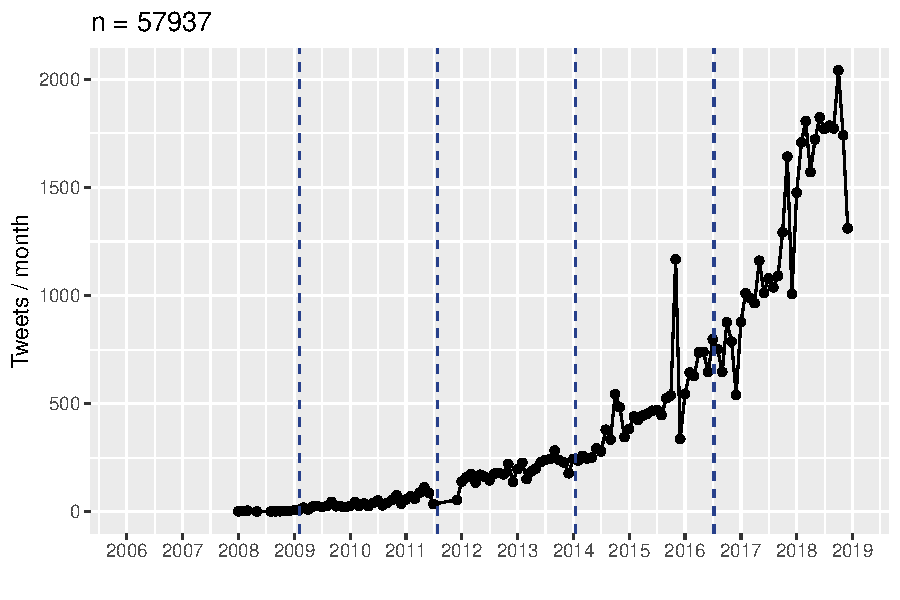
\includegraphics[width=\linewidth, height=.8\textheight, keepaspectratio]{"img/ui_upskill_time.pdf"}
        \end{subfigure}
        \hfill
        \begin{subfigure}{.3\linewidth}
          \caption{\ol{hyperlocal}}
          \label{subfig:freq_temp_hyperlocal}
          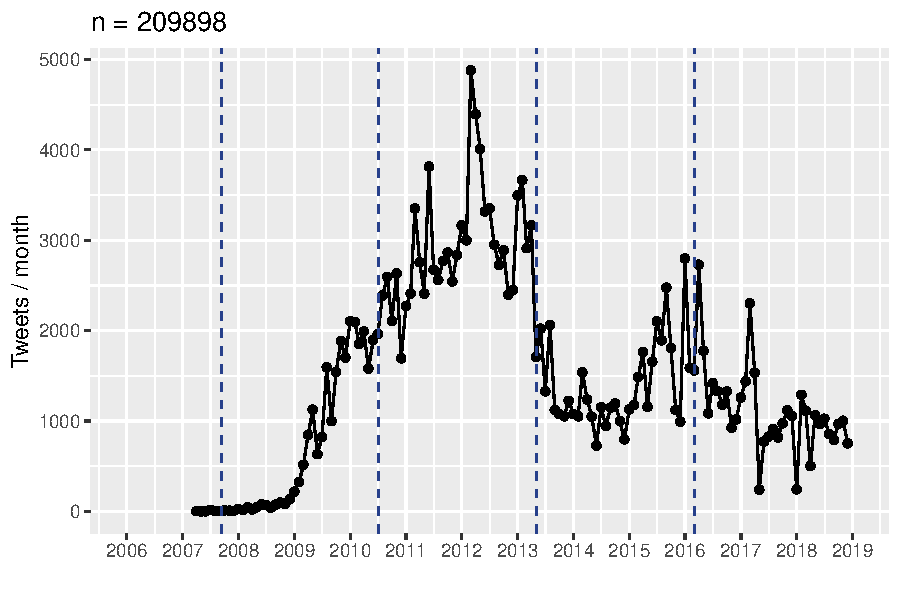
\includegraphics[width=\linewidth, height=.8\textheight, keepaspectratio]{"img/ui_hyperlocal_time.pdf"}
        \end{subfigure}
        \hfill
        \begin{subfigure}{.3\linewidth}
          \caption{\ol{solopreneur}}
          \label{subfig:freq_temp_solopreneur}
          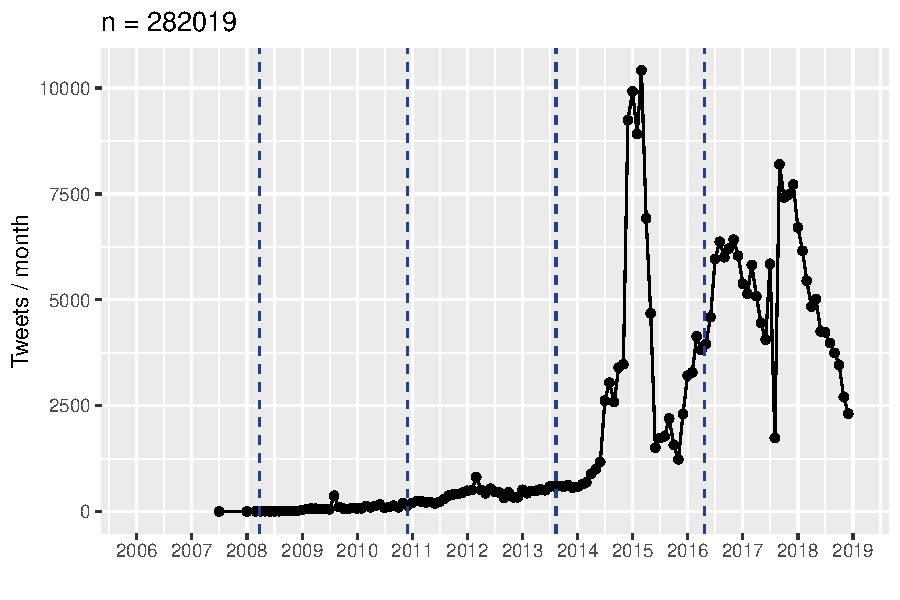
\includegraphics[width=\linewidth, height=.8\textheight, keepaspectratio]{"img/ui_solopreneur_time.pdf"}
        \end{subfigure}

        \begin{subfigure}{.3\linewidth}
          \caption{\ol{alt-right}}
          \label{subfig:freq_temp_alt-right}
          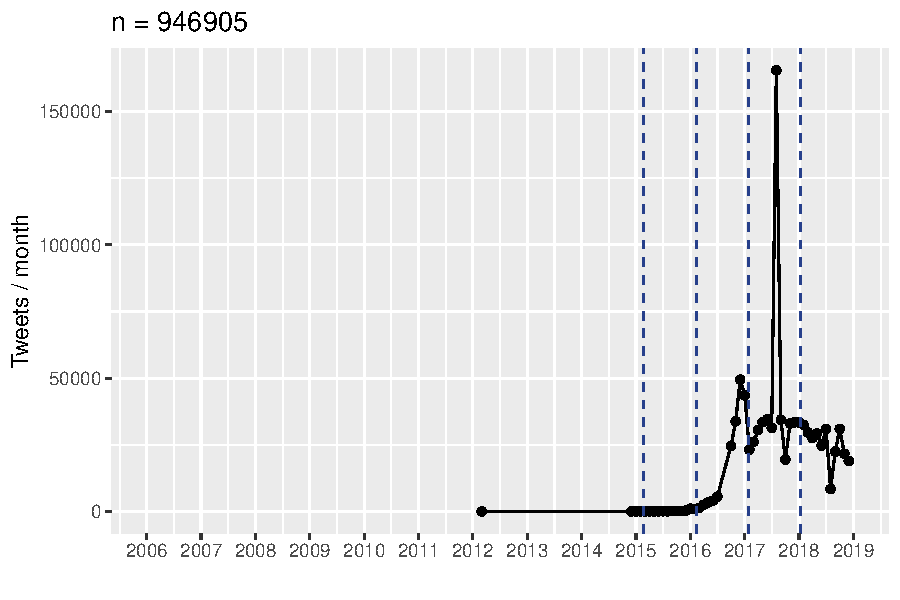
\includegraphics[width=\linewidth, height=.8\textheight, keepaspectratio]{"img/ui_alt-right_time.pdf"}
        \end{subfigure}
        \hfill
        \begin{subfigure}{.3\linewidth}
          \caption{\ol{alt-left}}
          \label{subfig:freq_temp_alt-left}
          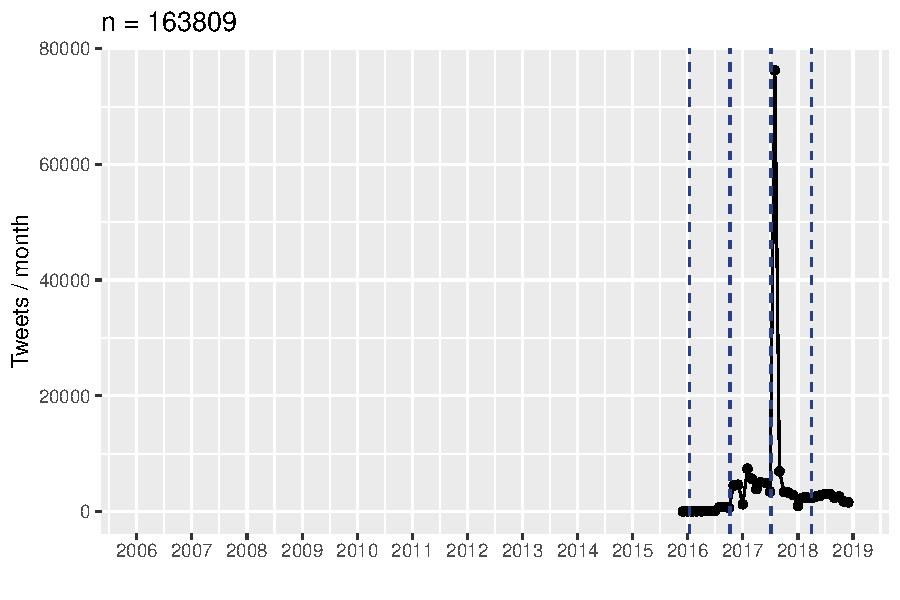
\includegraphics[width=\linewidth, height=.8\textheight, keepaspectratio]{"img/ui_alt-left_time.pdf"}
        \end{subfigure}
        \hfill
        \begin{subfigure}{.3\linewidth}
          \caption{\ol{poppygate}}
          \label{subfig:freq_temp_poppygate}
          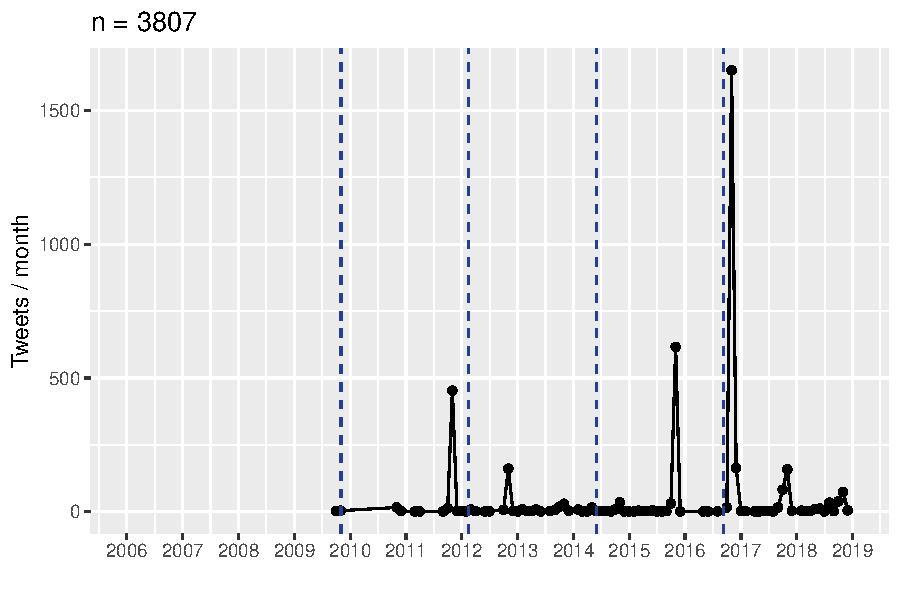
\includegraphics[width=\linewidth, height=.8\textheight, keepaspectratio]{"img/ui_poppygate_time.pdf"}
        \end{subfigure}
      \end{figure}

      The absolute frequency plots confirm differences regarding the lifespan and dynamics of usage intensity among the neologisms discussed above. In terms of lifespan, Figure \ref{fig:freq-abs} shows that \ol{upskill} and \ol{hyperlocal} are much older than \ol{alt-right} and \ol{alt-left}. The absolute counts also highlight the fact that while there is a low level of use of \ol{solopreneur} since 2007, its main period of diffusion starts much later, in 2014, with a subsequent spike in usage intensity.

      \qpar{Volatility}

        Besides, the absolute frequency counts over time provide a more detailed picture of the temporal dynamics of use. While the cumulative counts in Figure \ref{fig:freq_cum_cases} suggest smooth trajectories, the plots in Figure \ref{fig:freq-abs} indicate that the selected neologisms differ significantly in terms of the consistency with which they are used in the corpus.

        \marginpar{gradual increase} The neologism \ol{upskill} shows the smoothest trajectory of diffusion among the candidate neologisms. Aside from two smaller spikes, at the end of 2016 and 2018, it has gradually increased in its use since its first attestation in the corpus at the end of 2007. Neither its frequency counts, nor the corpus data suggest that its spread was triggered or propagated by specific topical events or the determining influence of individual influential users or user groups. After a long period of very slow, but consistent increase in frequency, its diffusion has accelerated in recent years. While its future remains uncertain, its previous trajectory resembles most closely the earlier phases of spread as predicted by S-curve models.

        \marginpar{consistent use} While \ol{hyperlocal} also exhibits a marked increase in usage frequency during its earlier stages, its peak of popularity is followed by a decline in use, after which it settles at a relative stable level of about \num{1000} tweets per month. This coincides with the OED's decision to take up \ol{hyperlocal} in its 2015 edition. Despite fluctuations, \ol{hyperlocal} has been used relatively consistently in the recent past, and seems to attract a stable community of users on Twitter.

        \marginpar{inconsistent use} The neologisms \ol{solopreneur} has been in use since 2007 and shows an overall increase in usage frequency, but its use fluctuates more strongly than that of \ol{hyperlocal}. After its initial peak around 2015, which coincides with the release of several self-help books featuring the term, its frequency plummets, becomes less stable, and shows an overall downward trend.

        \marginpar{topicality} As was mentioned above, \ol{alt-right} and \ol{alt-left} are closely related. Both terms show high levels of volatility in their usage frequency. The former, older term showed significant diffusion in 2016, particularly in the period following up to Donald Trump's election, after which \ol{alt-right} was consistently used to a relatively high degree, at about \num{25000} tweets per month. Its counterpart, \ol{alt-left}, enters the scene much later, during the infamous Charlottesville Rally in 2017, whose topical effect causes a huge spike in the use of both terms. However, unlike \ol{alt-right}, which returns to its previous usage intensity, the use of \ol{alt-left} seems to largely disappear from Twitter in the aftermath of the event.

        \marginpar{recurrent topicality} The last example among the selected candidates, \ol{poppygate}, also exhibits high degrees of volatility, and it features the most distinctive pattern of spikes in its usage intensity. Unlike the single topical spike for \ol{alt-right} and \ol{alt-left}, its use follows a recurrent, regular pattern: speakers use it almost exclusively around Remembrance Day, which takes place in November. The term \ol{poppygate} represents a last category of neologisms in the sample, which show wide fluctions in usage intensity, but for which these patterns follow a regular temporal pattern. \marginpar{\enquote{topicality}~\parencite{Fischer1998LexicalChange}; \enquote{recurrent semi-conventionalization}~\parencite{Kerremans2015WebNew})}


    \subsubsection{Coefficient of variation}
      \label{subsubsec:coef-var}

      To quantify the degree to which neologisms are used with consistent frequency over time, I calculate and compare the coefficients of variation for each neologism in the sample. This metric captures the overall variation in usage frequency of words over their lifespan relative to their average frequency of occurrence in the corpus. Table~\ref{tab:coef-var} presents the coefficients of variation for the selected neologisms, as well as for the top and bottom six neologisms that show the highest and lowest degrees of variation in the sample.

      \begin{table}
        \caption[Coefficient of variation]{Coefficients of variation (\textsc{var}) for the selected neologisms, and for six neologism with the highest and lowest scores in the sample.\protect\footnotemark}
        \label{tab:coef-var}
        \centering
        \begin{subtable}[t]{.3\linewidth}
          \caption{selected neologisms.}
          \label{subtab:coef-var-cases}
          \centering
          \begin{tabular}{
              l
              S[table-format=1.2, round-mode=places, round-precision=2]
            }
            \toprule
            Lexeme      & \textsc{var} \\
            \midrule
            hyperlocal  & 0.9783703    \\
            upskill     & 1.1399599    \\
            solopreneur	& 1.2046616    \\
            alt-right   & 1.8054940    \\
            poppygate   & 4.7535750    \\
            alt-left    & 5.3112621    \\
            \bottomrule
          \end{tabular}
        \end{subtable}
        \hfill
        \begin{subtable}[t]{.3\linewidth}
          \caption{Lowest scores.}
          \label{subtab:coef-var-lowest}
          \centering
          \begin{tabular}{
              l
              S[table-format=1.2, round-mode=places, round-precision=2]
            }
            \toprule
            Lexeme      & \textsc{var} \\
            \midrule
            followership  & 0.7147413 \\
            lituation     & 0.7174908 \\
            twitterverse  & 0.7215036 \\
            detweet       & 0.7436056 \\
            remoaners     & 0.7605029 \\
            twittersphere & 0.7670257 \\
            % baecation   & 0.7705697 \\
            % foodventure & 0.7714314 \\
            % broette     & 0.7726448 \\
            % upcycling   & 0.7995218 \\
            \bottomrule
          \end{tabular}
        \end{subtable}
        \hfill
        \begin{subtable}[t]{.3\linewidth}
          \caption{Highest scores.}
          \label{subtab:coef-highest}
          \centering
          \begin{tabular}{
              l
              S[table-format=1.2, round-mode=places, round-precision=2]
            }
            \toprule
            Lexeme      & \textsc{var} \\
            \midrule
            upskirting    & 9.3861492 \\
            youthquake    & 6.3218380 \\
            alt-left      & 5.3112621 \\
            birther       & 5.0001924 \\
            poppygate     & 4.7535750 \\
            cherpumple    & 4.6909168 \\
            % climate     & 14752     \\
            % incel       & 3.0090748 \\
            % neckbuds    & 2.9861481 \\
            % bloggergate & 2.7765687 \\
            \bottomrule
          \end{tabular}
        \end{subtable}
      \end{table}
      \footnotetext{Neologisms with a lifespan shorter than one year and/or less than \num{2000} tweets ($n = 5$) were excluded since the coefficient of variation does not provide robust measures for these short-lived, infrequent outliers.}

      The results in Table~\ref{tab:coef-var} show that the sample covers a wide spectrum of variability in usage frequency.

      Among the neologisms that were used the most consistently, i.e. exhibit the lowest degrees of variation, we find words whose frequency-based measures suggested high degrees of conventionality. For example, \ol{twitterverse} is listed among the most frequent neologisms in Table~\ref{subtab:freq-total-max} and is also one of the oldest neologisms, with its first attestation in the corpus dating back to 19 December, 2006.

      By contrast, the group of lexemes that show the highest degree of variation in usage frequency is comprised by neologisms with lower degrees of conventionality, which are generally less frequent and were coined more recently. Notably, topical spikes play a crucial role in the diffusion processes of all examples in this category: the diffusion of \ol{alt-left} and \ol{birther}\footnote{\enquote{proponent of the \enquote{birther movement}, a conspiracy theory which claims that President Obama's birth certificate was forged, and that he was not born in the USA.}} was promoted by extralinguistic political events, \ol{upskirting}\footnote{\mn{The habit or practice of taking upskirt photographs or videos.} (OED)} and \ol{youthquake}\footnote{\mn{a significant cultural, political, or social change arising from the actions or influence of young people} (\url{https://languages.oup.com/word-of-the-year/2017/})} were advanced through increased metalinguistic salience after they were added to the OED and awarded Word of the Year 2017 by Oxford University Press. Both \ol{poppygate} and \ol{cherpumple}\footnote{\mn{Cherpumple is short for cherry, pumpkin and apple pie. The apple pie is baked in spice cake, the pumpkin in yellow and the cherry in white.} (\url{https://en.wikipedia.org/wiki/Cherpumple}); typically consumed during the holiday season in the US.} exhibit recurrent topicality, and are typically only used in the contexts of their seasonal relevance in autumn and winter.

      The selected neologisms cover the spectrum of variability in usage frequency found in the full sample of neologisms, and the coefficients of variation are in line with the previous analysis of the frequency-based time-series visualisations presented in Figure~\ref{fig:freq-abs}.


      \subsubsection{Summary of frequency-based measures}

        So far, I have used frequency-based visualisations and metrics to assess the degrees and pathways of diffusion of the neologisms in the sample. In a first step, I used the most common measure for assessing the conventionality of new words: their total frequency of occurrence in the corpus. In the following steps, I extended the frequency-based approach by including temporal information in the analysis. Zooming in on the temporal dynamics of use surfaced different pathways of diffusion. Notably, it revealed substantial differences in the diachronic usage profiles of neologisms with comparable total frequency.

        Within the group of selected neologisms, \ol{hyperlocal}, \ol{solopreneur}, and \ol{alt-left}, for example, would all be placed in the medium range of the conventionality continuum if grouped by total usage frequency alone, as presented in Table~\ref{subtab:freq-total-cases}. Taking this most basic measure as an indicator of degrees of diffusion, it would seem that these words are roughly equally conventional among users on Twitter. However, adding the temporal dynamics of their use in the corpus to the picture revealed significant differences between their diachronic usage profiles, which seems important for assessing their pathways and degrees of diffusion in a more differentiated and accurate way.

        Visualising the cumulative increase in uses over time (Table~\ref{fig:freq_cum_cases}) for \ol{hyperlocal}, for example, shows a stable linear trend, which indicates that its total frequency count has been the product of relatively consistent use over its relatively long lifespan. Its temporal usage profile in Figure~\ref{subfig:freq_temp_hyperlocal} and confirms these observations and presents its initial period of accelerated diffusion followed by an extended stable level of relatively consistent use over the last five years of its observed lifespan. This consistency is further corroborated by its low coefficient of variation (Table~\ref{subtab:coef-var-cases}). In sum, the balanced nature of this frequency-based usage profile suggests a relatively organic trajectory of diffusion, culminating in a solid degree of conventionality in the recent past. The fact that \ol{hyperlocal} was added to the OED in 2015 supports these observations.

        By comparison, \ol{solopreneur} has a slightly higher overall frequency of occurrence in the corpus, yet its use is less stable over time. While its overall lifespan is about as long as that of \ol{hyperlocal}, its cumulative distribution shows that the majority of its use goes back to a relative short period of intensive use, after which it exhibits a slightly negative trend in later stages. Both the visualization of its temporal frequency profile as well as its coefficient of variation demonstrate a higher degree of fluctuation in its popularity. This temporal usage pattern suggests that its diffusion was influenced significantly by effects of topical salience. While \ol{solopreneur} has been used in a high total number of tweets in the corpus, it thus seems less certain whether its use will become stable over time, and to which degree its use extends beyond the entrepreneurial community which triggered the main spurt of its diffusion in the second half of 2014.

        Lastly, \ol{alt-left} is in the same range of total usage frequency, but its use is much more unevenly dispersed across the corpus than that of the remaining selected neologisms. The term is much younger, and its cumulative increase in uses illustrates that diffusion is largely limited to a very short, highly intensive period of use, after which it shows a strong negativ trend in its usage frequency. Its diachronic frequency profile and its coefficient of variation correspondingly demonstrate very high levels of fluctuations in its use. Since the short period of intense use of \ol{alt-left} can clearly be traced back to participants of the Unite the Right Rally in Charlottesville in August 2017, it seems plausible that its popularity has never extended beyond this topical event and beyond this particular community of like-minded individuals.
        
        The frequency-based analysis of the three neologisms discussed above demonstrates that usage frequency counts, particularly when combined with an analysis of their underlying temporal dynamics, can help to approximate the spread and success of neologisms to a certain degree. However, the results also point to substantial limitations of frequency-based approaches to studying diffusion. The present data demonstrate high degrees of variation in the degrees of diffusion of neologims that are similar in terms of their frequency of occurrence in the corpus. Such discrepancies could partly be resolved by in-depth analyses of temporal usage profiles in combination with insights from corpus data and extralinguistic events. These in-depth analyses of diffusion are not possible by a systematic frequency-based analysis alone, however, and they cannot be extended for large-scale analyses of bigger samples of neologisms. It hence remains unknown to which degree frequency-based metrics adequately capture pathways and degrees of diffusion. In the following section, I will address the limitations of the frequency-based approach by using Social Network Analysis to get a more differentiated view on the sociolinguistic aspects of diffusion.


  \subsection{Social networks of diffusion}
    \label{subsec:sna}

    As discussed in Section~XXX, from a theoretical, sociolinguistic perspective, the degree of diffusion of lexical innovations depends on the degree to which new words become conventional among new speakers and communities of speakers. Frequency-based analyses, as presented in the previous section, can by definition only provide information about the distribution of occurrences of neologisms in the corpus, they cannot provide direct evidence about the size and composition of the community of speakers who have produced the observed attestations.

    Social network analysis, by contrast, is based on data about the communicative behaviour of speakers in the corpus and can thus provide direct insights into the social characteristics of the speech community. This allows for a more direct operationalization of the theoretical model of diffusion. The structural characteristics of the social network of speakers who have used a target neologism can be used to assess whether the term has been used by a broad section of the speech community, or whether its use remains limited to certain parts of the speech community.

    As described in Section~\ref{sec:method}, the social network analysis is based on the interactions between all speakers who have used the neologisms in the sample. Speakers are represented as nodes in the network graph, and interactions between users in the form of replies or mentions are represented as edges. The network structure of the resulting graphs allows to analyse the degree to which the target neologisms have diffused in these networks.

    To monitor diffusion over time, I split the observed lifespan of each neologism into four equally-sized time slices. These time windows are marked by dashed vertical lines in Figure~\ref{fig:freq-abs}. I then generate network graphs for each time window for each neologism in the sample to analyse the individual pathways of diffusion over time and to compare degrees of diffusion between all neologisms in the sample.

    \subsubsection{Degrees of diffusion}
      \label{subsec:degrees-of-diffusion}

      As discussed in Section~\ref{sec:method}, I mainly rely on degree centralization as a quantitative measure for degrees of diffusion. I consider increasing diffusion to be reflected by decreasing degree centralization of the graph, thus lower values of centrality indicate higher degrees of diffusion. For example, the social graph users of a new word shows high centralization in early stages when its use is largely confined to one or few centralized clusters of speakers. When increasing diffusion extends the use of the term to new speakers and communities, the distribution of interactions in the speech community shows greater dispersion, which should be reflected by lower centrality scores for the social network of speakers.

      Table~\ref{tab:cent_last_cases-sample} reports the degree centrality scores for the selected neologisms and for six lexemes with the highest and lowest scores in the sample.

      \begin{table}
        \caption[Degree centrality scores]{Degree centrality scores (\textsc{cent}) for the selected neologisms and six lexemes each for the highest and lowest scores in the sample; the scores are based on the last subset for each neologisms in the corpus.}
        \label{tab:cent_last_cases-sample}
        \begin{subtable}{.3\linewidth}
          \centering
          \caption{Selected neologisms.}
          \label{subtab:cent_last_cases}
          \begin{tabular}{l S[table-format=1.4, round-mode=places, round-precision=4]}
            \toprule
            Lexeme      & {\textsc{cent}} \\
            \midrule
            upskill     & 0.002061916  \\
            hyperlocal	& 0.008527674  \\
            alt-right   & 0.014425502  \\
            alt-left    & 0.023848081  \\
            solopreneur	& 0.052339695  \\
            poppygate   & 0.056645023  \\
            \bottomrule
          \end{tabular}
        \end{subtable}
        \hfill
        \begin{subtable}{.3\linewidth}
          \centering
          \caption{Lowest scores.}
          \begin{tabular}{l S[table-format=1.4, round-mode=places, round-precision=4]}
            \toprule
            Lexeme          & {\textsc{cent}} \\
            \midrule
            baecation       & 0.0005064777 \\
            fleek           & 0.0009416515 \\
            ghosting        & 0.0013446084 \\
            man bun         & 0.0015875456 \\
            big dick energy	& 0.0018204662 \\
            twittersphere   & 0.0019679891 \\
            \bottomrule
          \end{tabular}
        \end{subtable}
        \hfill
        \begin{subtable}{.3\linewidth}
          \centering
          \caption{Highest scores.}
          \begin{tabular}{l S[table-format=1.4, round-mode=places, round-precision=4]}
            \toprule
            Lexeme      & {\textsc{cent}} \\
            \midrule
            rapugee     & 0.2579569224 \\
            levidrome   & 0.2372565853 \\
            Kushnergate	& 0.2308673469 \\
            dronography	& 0.1530180700 \\
            dotard      & 0.0978663785 \\
            ecocide     & 0.0921670083 \\
            \bottomrule
          \end{tabular}
        \end{subtable}
      \end{table}

      The neologisms with the lowest scores for degree centrality are also among the most frequent lexemes in the sample. This indicates that frequency and centrality generally tend to produce similar results when used to assess degrees of diffusion, which seems to cross-validate both approaches to some degree. Notable deviations exist, however, and will be further discussed in Section~\ref{subsec:nets-vs-freq}.

      Correspondingly, the neologisms with the highest centrality scores rank among the least frequent example. Notable trends among lexemes with low centrality scores are that they tend to be more recent (e.g. \ol{dronography}\footnote{\enquote{Dronography is the science, art and practice of creating durable images or video by recording light or other electromagnetic radiation by means of a drone flying around or above a certain scene} (Urban Dictionary).}) and/or to exhibit high degrees of topical variation (e.g. \ol{ecocide}\footnote{\enquote{the destruction of large areas of the natural environment as a consequence of human activity} (Merriam Webster Online Dictionary).}). Moreover, this groups includes political terms such as \ol{Kushnergate}\footnote{Referring to a political scandal involving Trump's senior adviser Jared Kushner allegedly meeting Russian officials.} and \ol{rapugee} which are controversially discussed on the left and right ends of the political spectrum. For example, \ol{rapugee} is a derogatory term which was coined after sexual assaults by refugees during New Year's Eve 2015/16 in Cologne, Germany. Previous work has shown that this term was consciously coined and propagated by a closely connected community of far-right activists to disparage refugees, and that its use on Twitter and on the Web has remained largely limited to these communities \parencite{Wurschinger2016UsingWeb}. This low degree of diffusion is reflected by the low centrality score for \ol{rapugee}.

      The centrality scores for the selected neologisms cover a broad spectrum of degrees of diffusion, as can be seen in Table~\ref{subtab:cent_last_cases}. Figure~\ref{fig:net_last_cases} presents the full network graphs for four of the selected cases to illustrate differences in the social networks of speakers which are captured by centrality scores.\footnote{The network graphs for \ol{alt-right} and \ol{poppygate} were omitted as their difference in network size does not allow for comparative analyses (\ol{alt-right}: \num{274686} nodes, \ol{poppygate}: \num{2473} nodes).}  

      \begin{figure}
        \captionsetup[subfigure]{justification=centering}
        \caption[Social networks of diffusion for the selected neologisms]{Social network graphs for the last subset of the selected neologisms.}
        \label{fig:net_last_cases}
        \centering
        \begin{subfigure}{.45\linewidth}
          \caption{\se{\ol{upskill}}\\ (\num{37044}~nodes, \num{23060}~edges)}
          \label{subfig:net_last_cases_upskill}
          % \includegraphics[width=\linewidth]{example-image-a}
          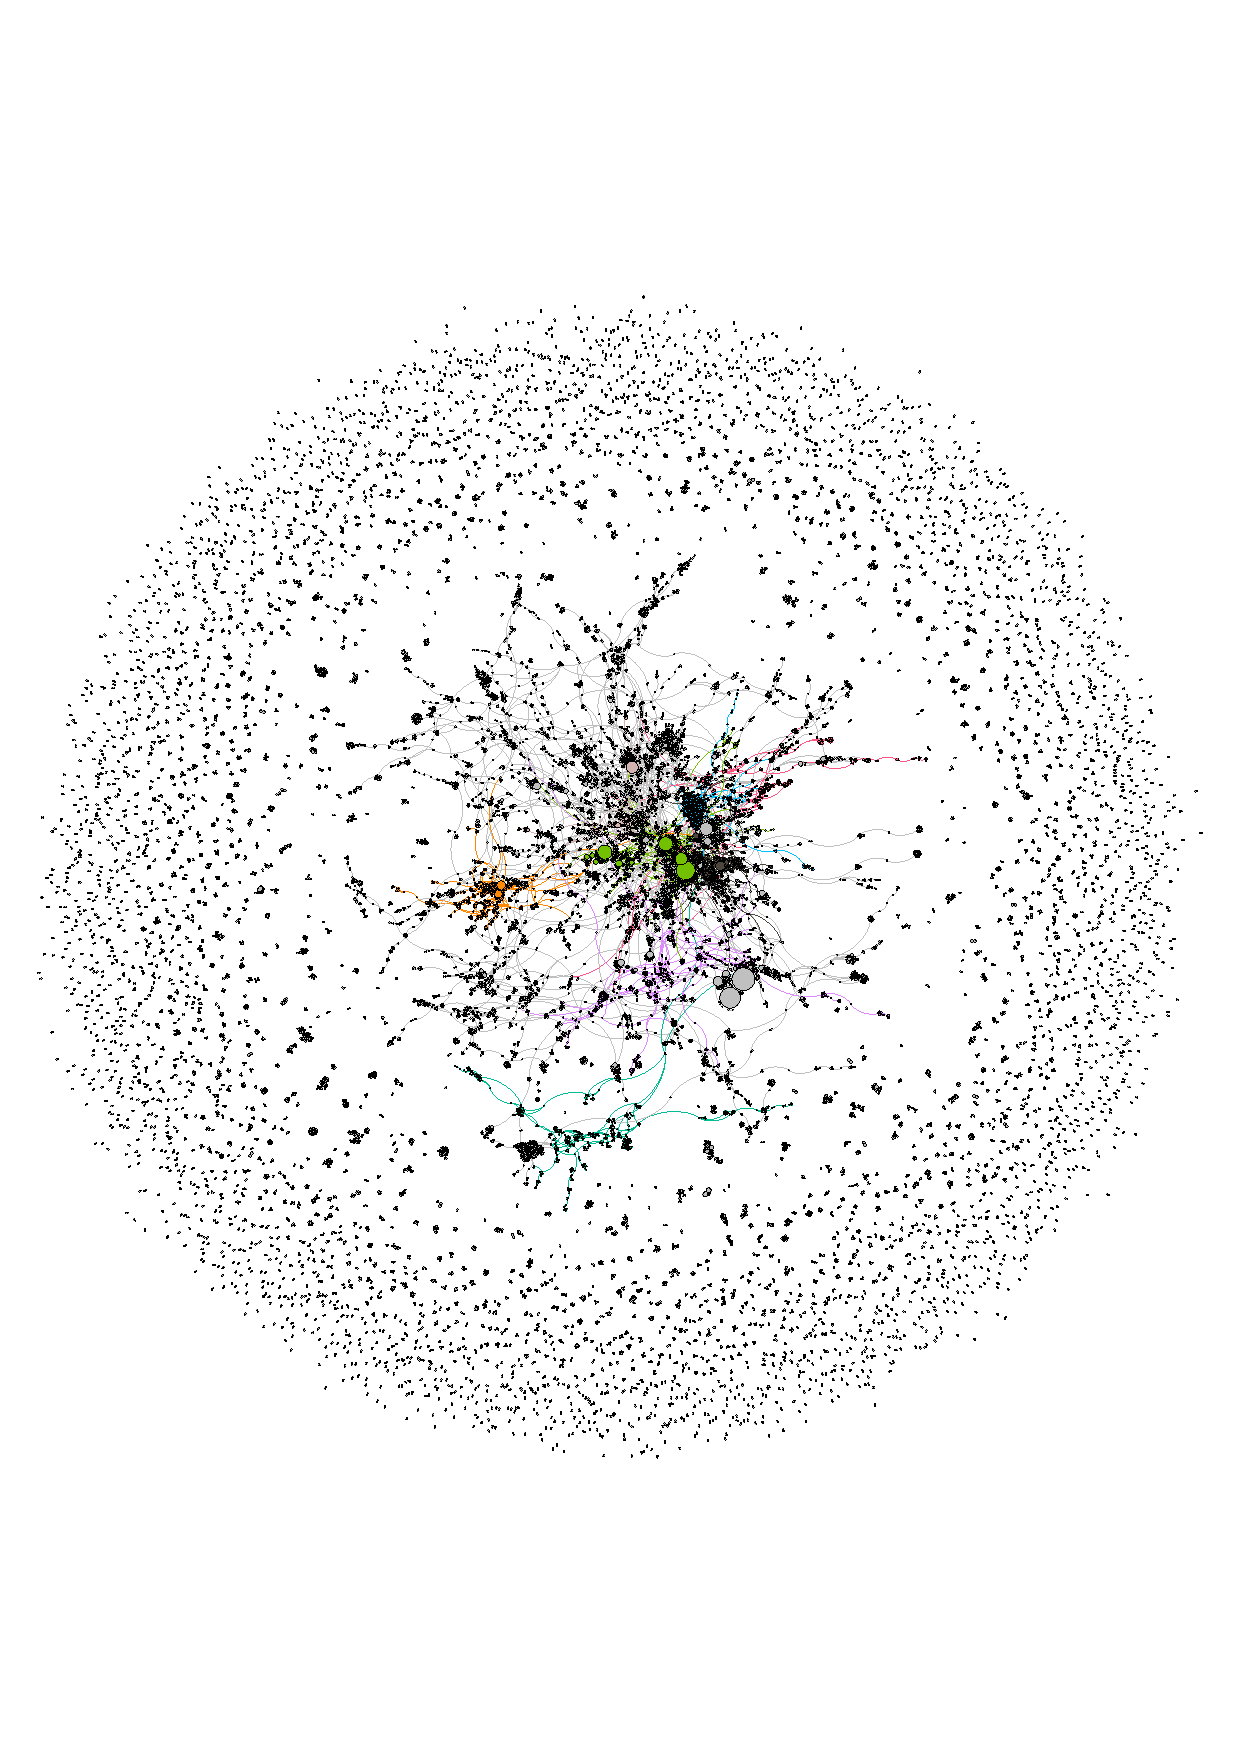
\includegraphics[width=\linewidth, height=\textheight, keepaspectratio]{img/net_upskill_four.pdf}
        \end{subfigure}
        \begin{subfigure}{.45\linewidth}
          \caption{\se{\ol{hyperlocal}}\\ (\num{26548}~nodes, \num{16576}~edges)}
          \label{subfig:net_last_cases_hyperlocal}
          % \includegraphics[width=\linewidth]{example-image-b}
          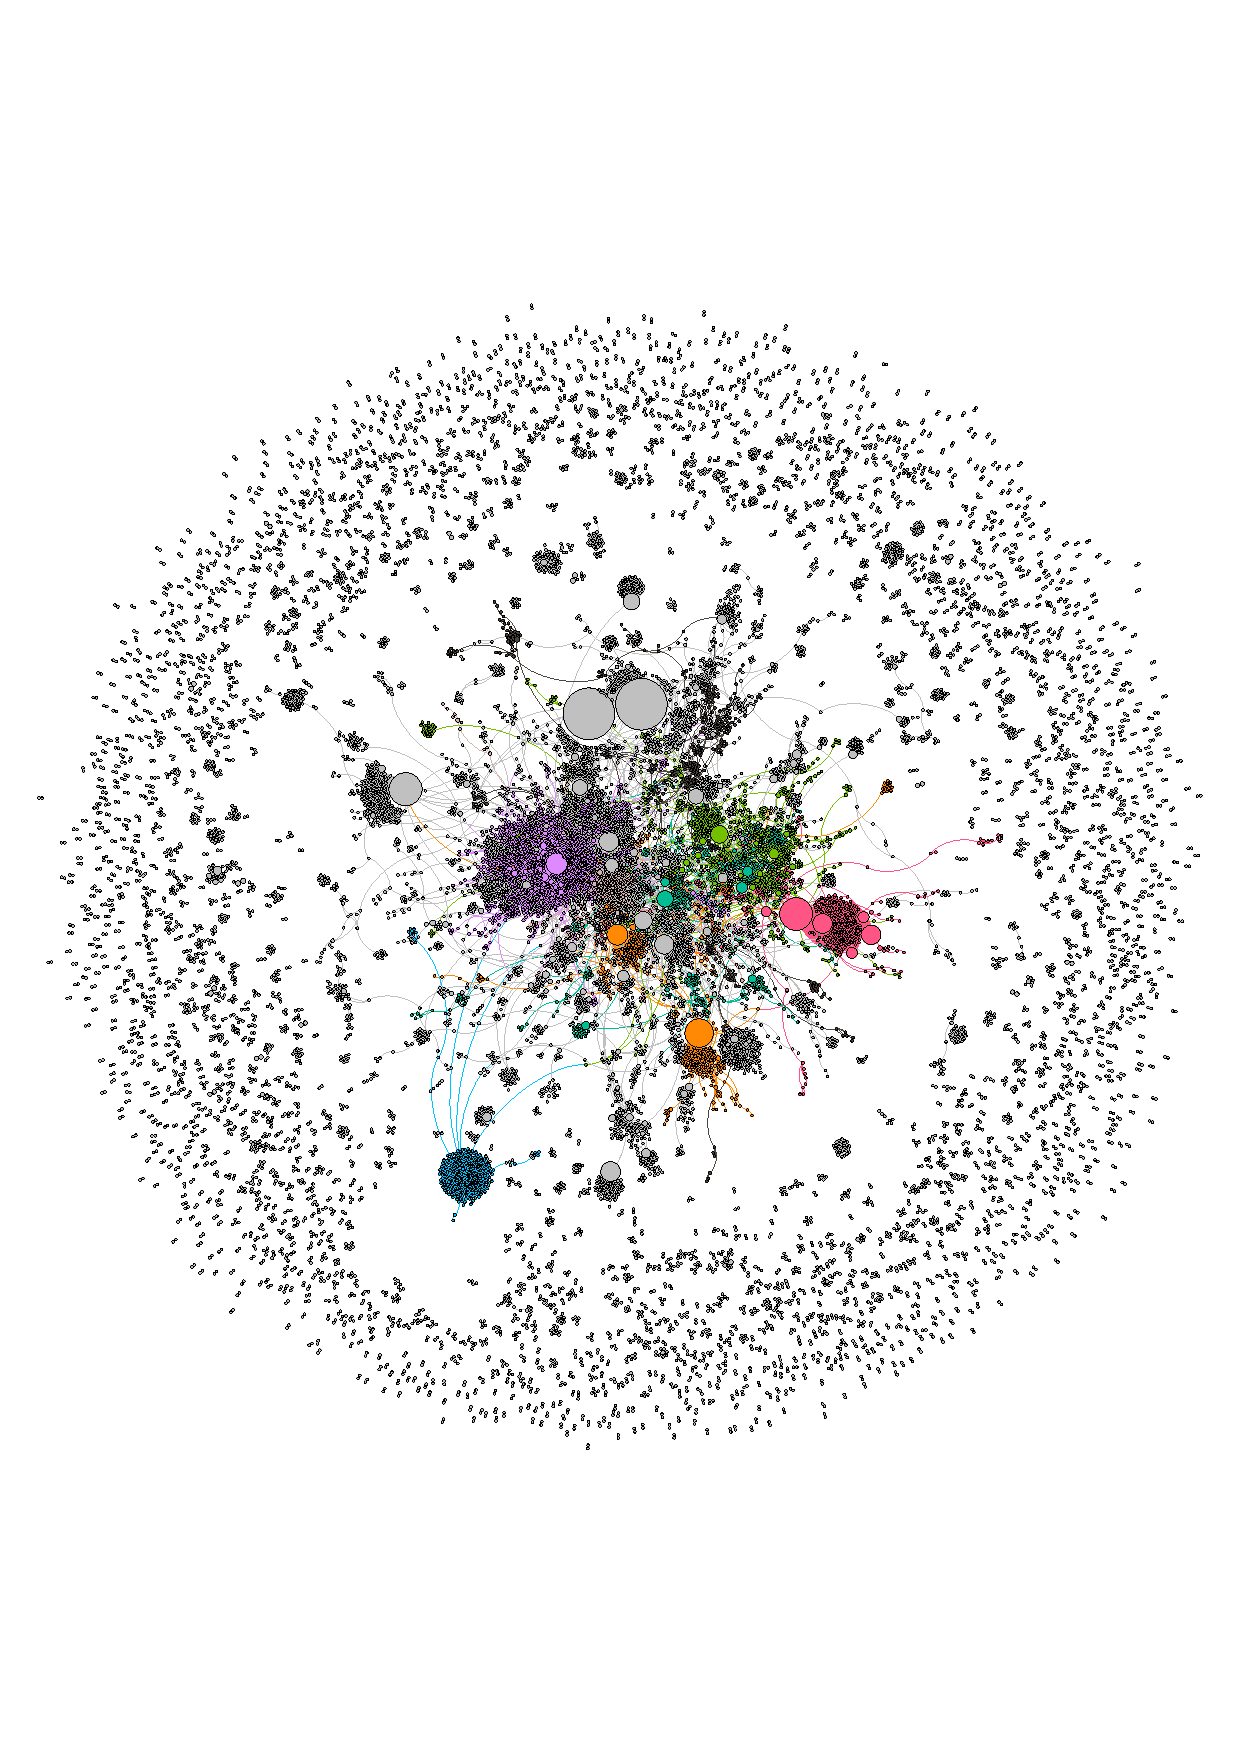
\includegraphics[width=\linewidth, height=\textheight, keepaspectratio]{img/net_hyperlocal_four.pdf}
        \end{subfigure}

        \begin{subfigure}{.45\linewidth}
          \caption{\se{\ol{alt-left}}\\ (\num{26367}~nodes, \num{32836}~edges)}
          \label{subfig:net_last_cases_alt-left}
          % \includegraphics[width=\linewidth]{example-image-a}
          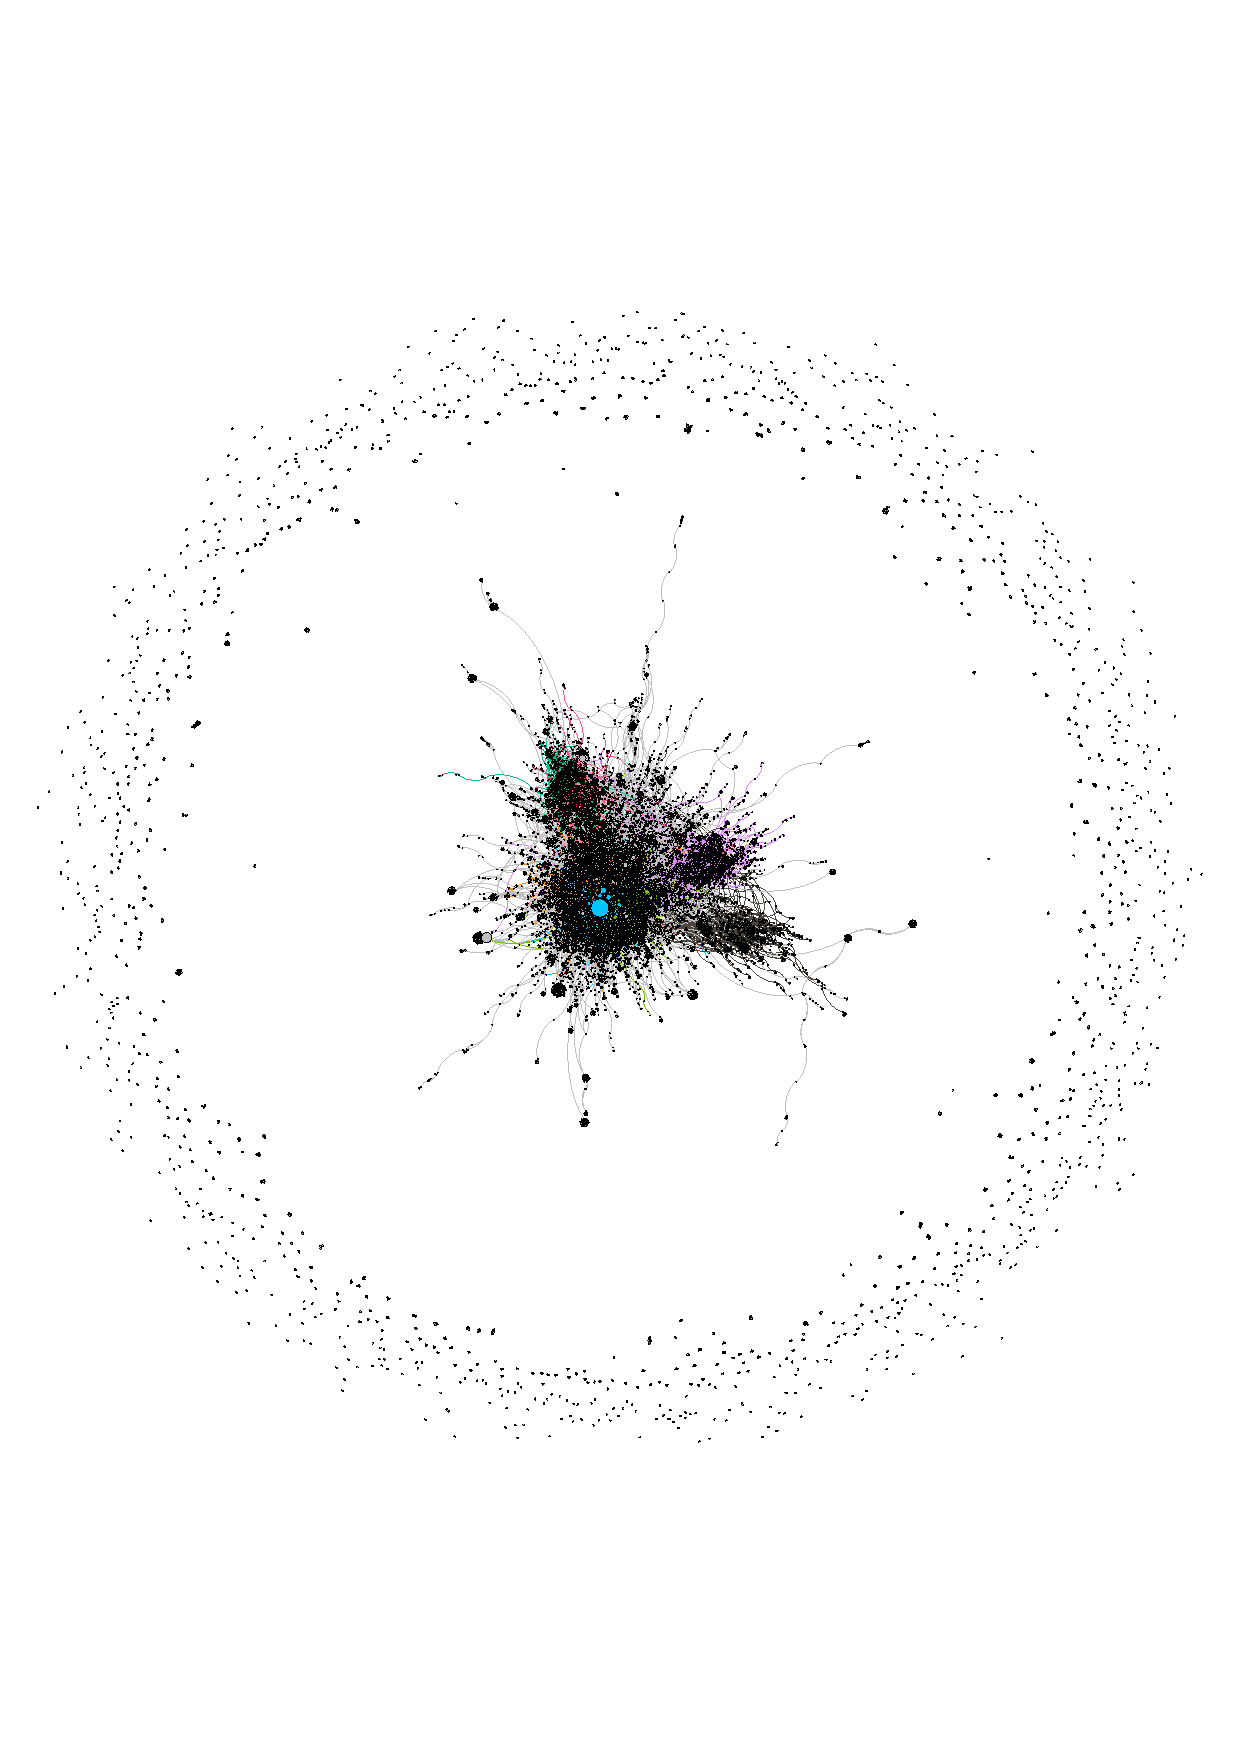
\includegraphics[width=\linewidth, height=\textheight, keepaspectratio]{img/net_alt-left_four.pdf}
        \end{subfigure}
        \begin{subfigure}{.45\linewidth}
          \caption{\se{\ol{solopreneur}}\\ (\num{24585}~nodes, \num{20486}~edges)}
          \label{subfig:net_last_cases_solopreneur}
          % \includegraphics[width=\linewidth]{example-image-c}
          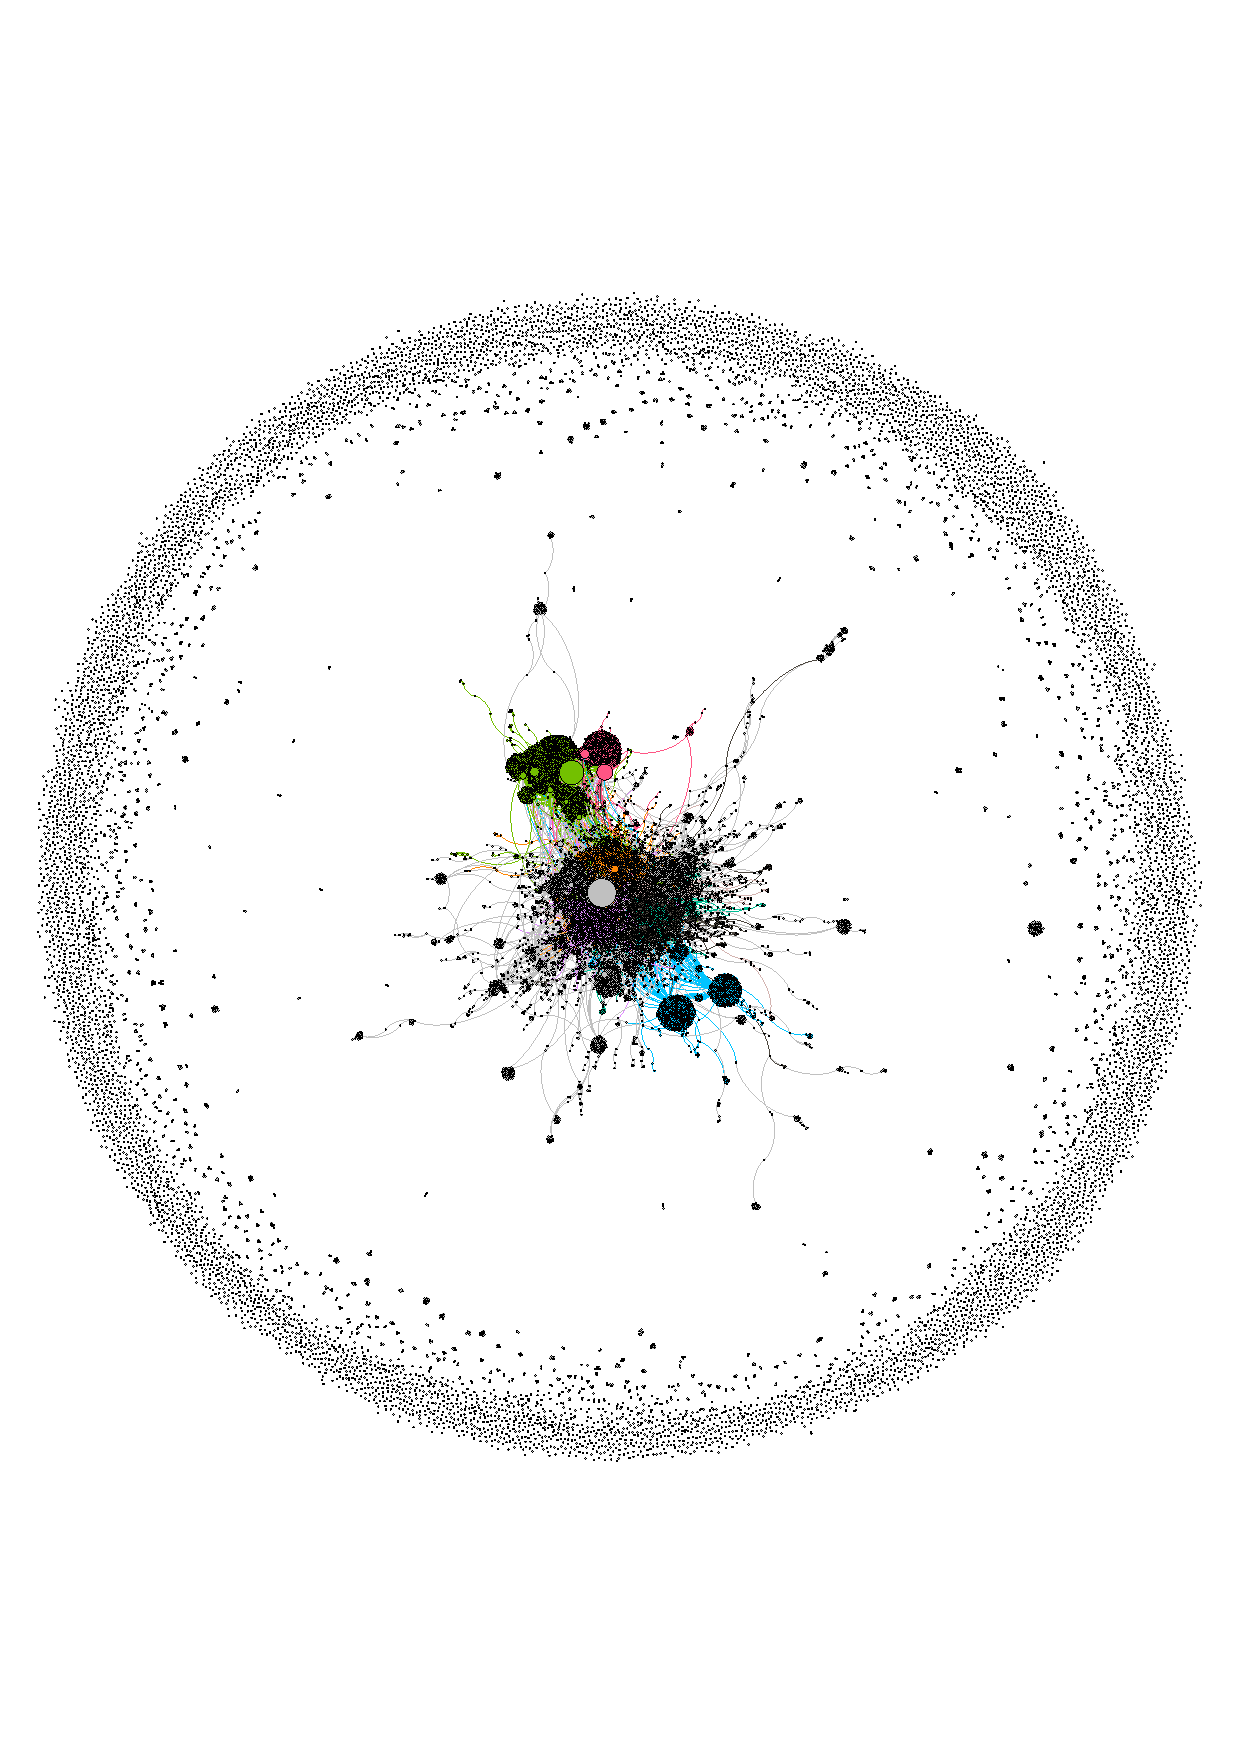
\includegraphics[width=\linewidth, height=\textheight, keepaspectratio]{img/net_solopreneur_four.pdf}
        \end{subfigure}
      \end{figure}

      The network graphs in Figure~\ref{fig:net_last_cases} are sorted according to their degrees of diffusion -- as measured by centrality scores -- from (a) to (d). Note that the number of nodes in each graph is very similar, differences between network graphs are thus due to differences in the underlying social structure of communities rather than a mere function of differences in network size.

      The neologisms \ol{upskill} exhibits the highest degree of diffusion, which is reflected by the highest degree of dispersion of nodes across the graph in Figure~\ref{subfig:net_last_cases_upskill}. At the center of the graph, we find a relatively large community of speakers who are only loosely connected. Many of these speakers are connected via their affiliations to the world of business, where the term \ol{upskill} is most commonly used. However, the use of the term can not be traced back to a small set of densely connected communities. As the high proportion of nodes towards the fringes of the graph reveals, most occurrences of the term are produced by speakers who use the term independently of associations to specific communities. 

      The graph for \ol{hyperlocal} in Figure~\ref{subfig:net_last_cases_hyperlocal} also shows a high degree of diffusion, but its use depends more strongly on a central community of users. This core sub-network of speakers forms several smaller clusters which can be linked to certain domains of interest such as journalism, business, and startups, in which the term is most popular. Notably, we observe a stronger role of individual user accounts such as influencers and marketing agencies, which is illustrated by bigger node sizes, which represent PageRank scores. Yet, as in the graph for \ol{upskill}, the majority of occurrences of \ol{hyperlocal} can be traced back to a high number of speakers from a diverse set of sub-communities, which can be interpreted as a sign of advanced diffusion.

      The social graph for \ol{alt-left} shows very limited diffusion of the term. Almost all of its use can be traced back to one central community of users. This core community of users demonstrates typical characteristics of an echo chamber in that it is dense and features strong ties within the community, but is isolated and has few weak ties connecting it to the rest of the social graph. This observation is in line with the socio-political background of the term, which was coined and propagated by far-right activists in an attempt to unify political efforts (\enquote{\emph{Unite} the Right Rally}) and to distance themselves and protest against the political left. Inspecting the network reveals that the most influential node in the network is Donald Trump, whose use of the term was followed by a sharp increase in usage intensity in the course of the Charlottesville Rally in August 2017. The high degree of social fragmentation in the use of \ol{alt-left} is also reflected in the ration between the number of nodes and edges in its graph, which confirms that its community of speakers is much more closely connected than that of the remaining neologisms\footnote{The numbers of edges per node for all selected cases in descending order: \ol{alt-right}: \num{1.49}, \ol{alt-left}: \num{1.24}, \ol{solopreneur}: \num{0.83}, \ol{hyperlocal}: \num{0.62}, \ol{upskill}: \num{0.62}, \ol{poppygate}: \num{0.53}}. Notably, the same applies to the community of \ol{alt-right}, which occupies the opposite pole of the political spectrum, which seems in line with effects of political polarization in social networks observed in previous work~\parencite{Sunstein2018RepublicDivided}. Overall, \ol{alt-left} thus shows a low degree of diffusion. It has received significant popularity in certain parts of the speech community, but its use remains strongly limited to these communities.

      Lastly, the social network of speakers using the term \ol{solopreneur} also shows a low degree of diffusion. A significant proportion of its use comes from a diverse set of individual speakers and micro-communities, which are placed at the fringes of the graph. However, a relatively well-connected, large core of speakers is responsible for the majority of its use in the corpus. Moreover, unlike the example of \ol{alt-left}, this central community of users is in turn dominated by the high centrality of a small number of individual accounts. Inspecting the network of users reveals that these \enquote{influencers} are all either proud, self-proclaimed solopreneurs, or coaches and agencies that are using the term to promote their services to aspiring entrepreneurs. Overall, \ol{solopreneur} thus shows a low degree of diffusion. It has achieved significant popularity within certain communities, but its use in these communities is unevenly distributed and depends strongly on a small number of individual users. The term does not show signs of advanced diffusion since its use does only extend beyond certain individual speakers and subcommunities to a very limited degree.

      In summary, the social networks of speakers reveal significant differences in the degrees of diffusion for the neologisms in the sample. While the centrality measures generally concur with the results obtained from the frequency-based analysis in Section~\ref{subsec:freq}, the network metrics and visualisation provide a more detailed picture of degrees of social diffusion and highlights certain cases, for which the social dynamics of diffusion diverge from what could be observed by relying on usage frequency alone.


    \subsubsection{Pathways of diffusion}

      The following section will extend the present analysis of degrees of diffusion to investigate the development of social diffusion over time. Figure~\ref{fig:cent_diac_cases} presents the degree centrality scores for the selected neolgisms over time. While the scores for Subset 4 represent the final degrees of diffusion for these terms as presented in Table~\ref{subtab:cent_last_cases} and which are based on the network graphs illustrated in Figure~\ref{fig:net_last_cases}, the previous subsets provide information about their diffusion history. The diverging trajectories of centralization over time indicate significant changes over time as well als differences in the pathways of diffusion between neologisms.

      \begin{figure}
        \caption[Centralization over time for the selected neologisms]{Pathways of diffusion for the selected neologisms. The graph shows \textsc{degree centrality} scores over time, each \textsc{subset} representing one network graph which was generated for each of the four equally-sized time slices for each neologism in the sample.}
        \label{fig:cent_diac_cases}
        \centering
        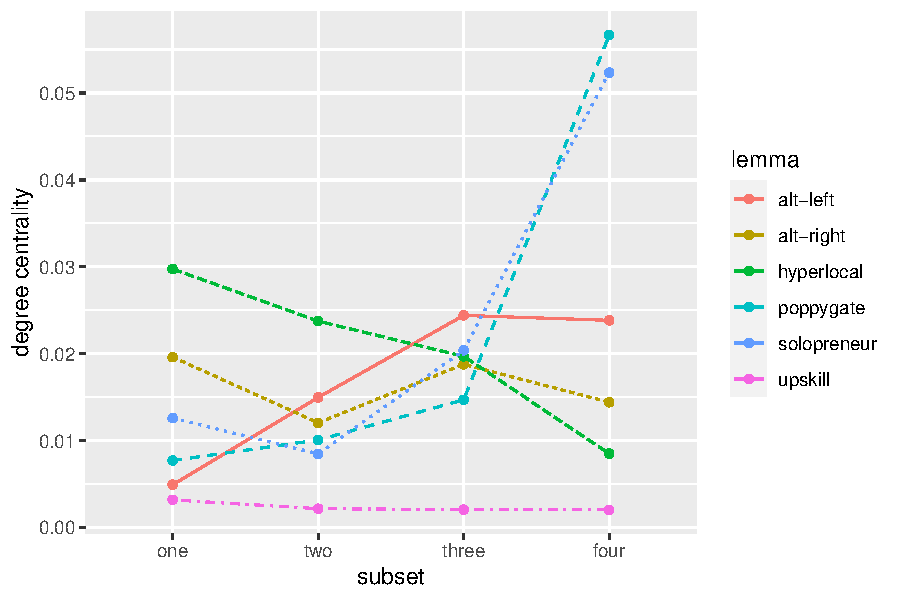
\includegraphics[width=\linewidth, height=.8\textheight, keepaspectratio]{img/cases_cent_diac.pdf}
      \end{figure}

      Before I discuss the results for all selected cases, I will present the full network graphs for all stages of diffusion of \ol{hyperlocal} (\ref{fig:net_diac_hyperlocal}) to illustrate the social dynamics underlying the quantitative measures.

      \begin{figure}
        \captionsetup[subfigure]{justification=centering}
        \centering
        \begin{subfigure}{.45\linewidth}
          \caption{\se{Subset 1}\\ 10~Sept,~2007 -- 8~Jul~2010;\\ nodes: \num{12569}, edges: \num{13742}}
          \label{subfig:net_diac_hyperlocal_one}
          \centering
          % \includegraphics[width=\linewidth]{example-image-a}
          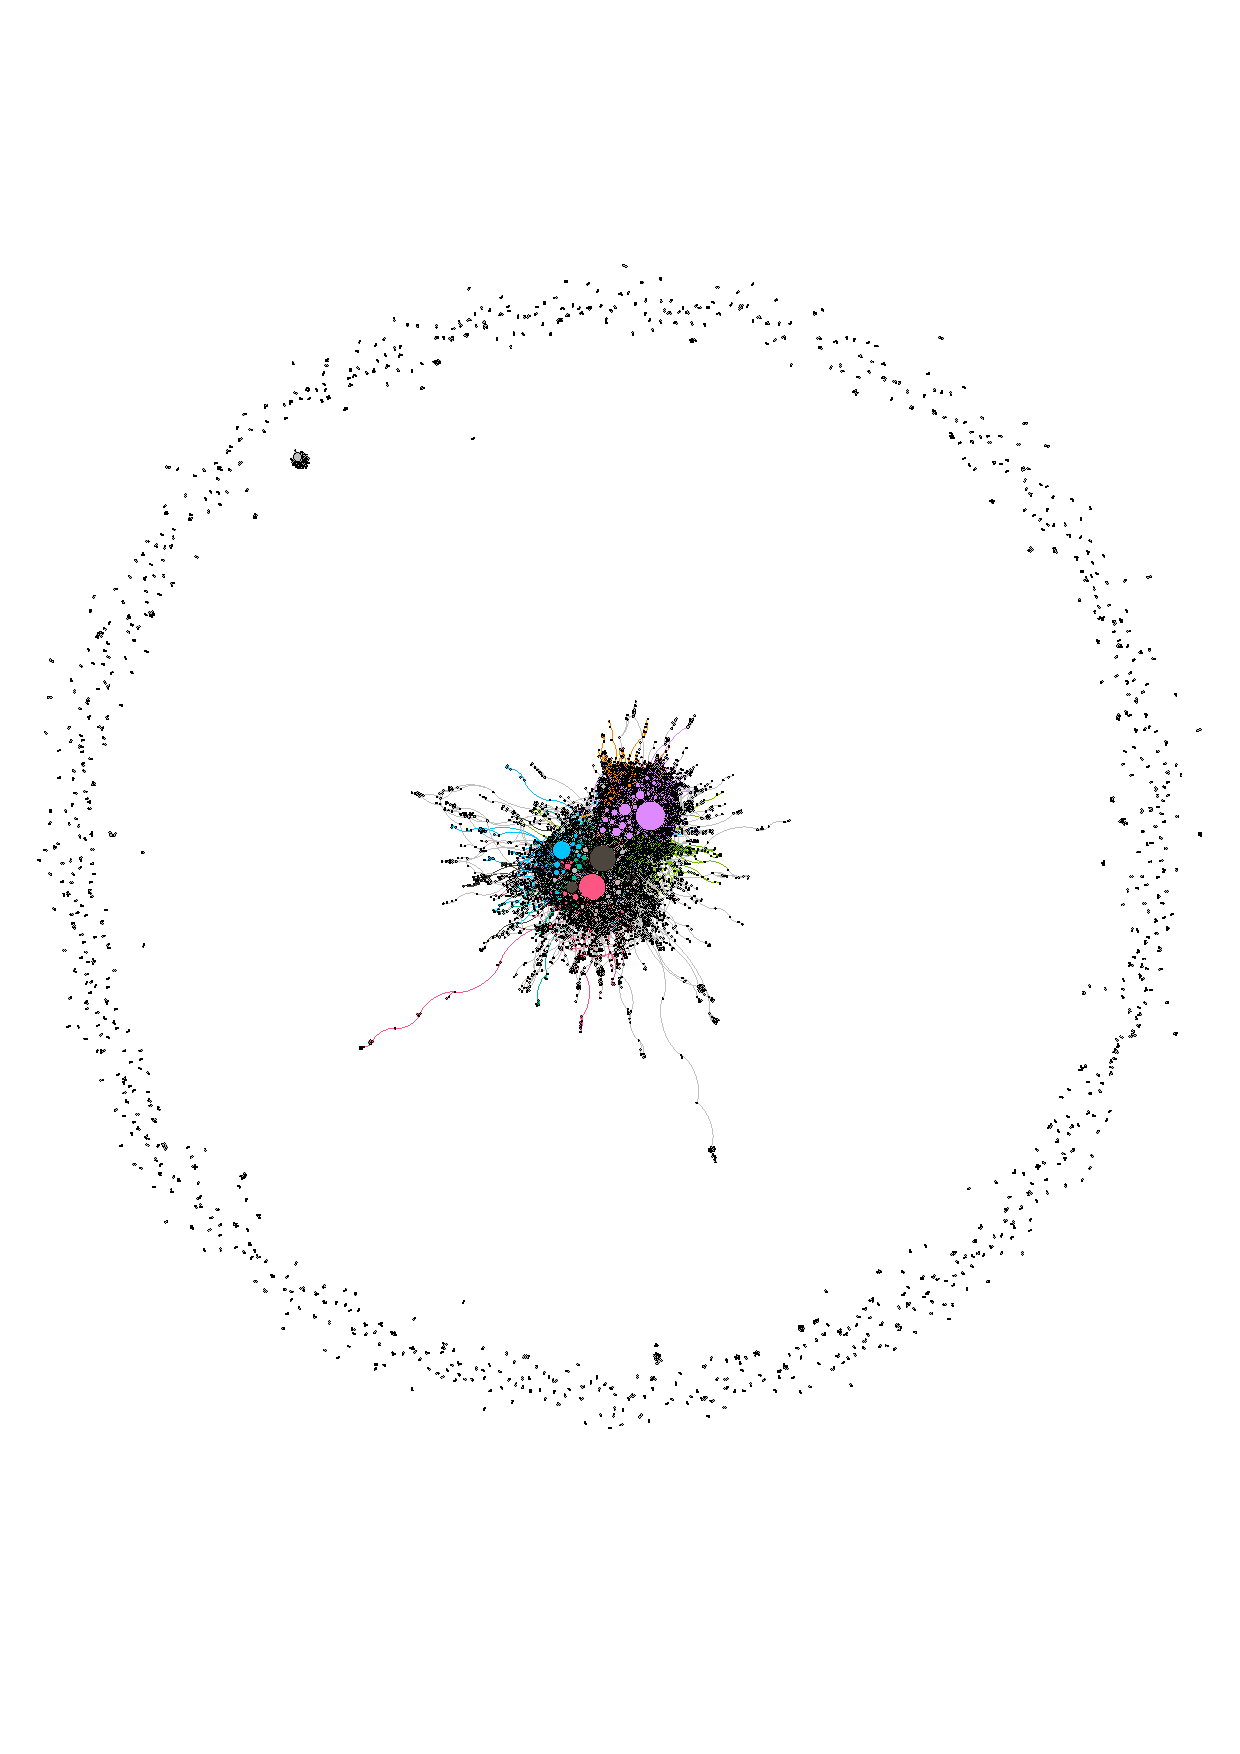
\includegraphics[width=\linewidth, height=\textheight, keepaspectratio]{img/net_hyperlocal_one.pdf}
        \end{subfigure}
        \begin{subfigure}{.45\linewidth}
          \caption{\se{Subset 2}\\ 9~Jul.,~2010 -- 5~May,~2013;\\ nodes: \num{33450}, edges: \num{34109}}
          \label{subfig:net_diac_hyperlocal_two}
          \centering
          % \includegraphics[width=\linewidth]{example-image-b}
          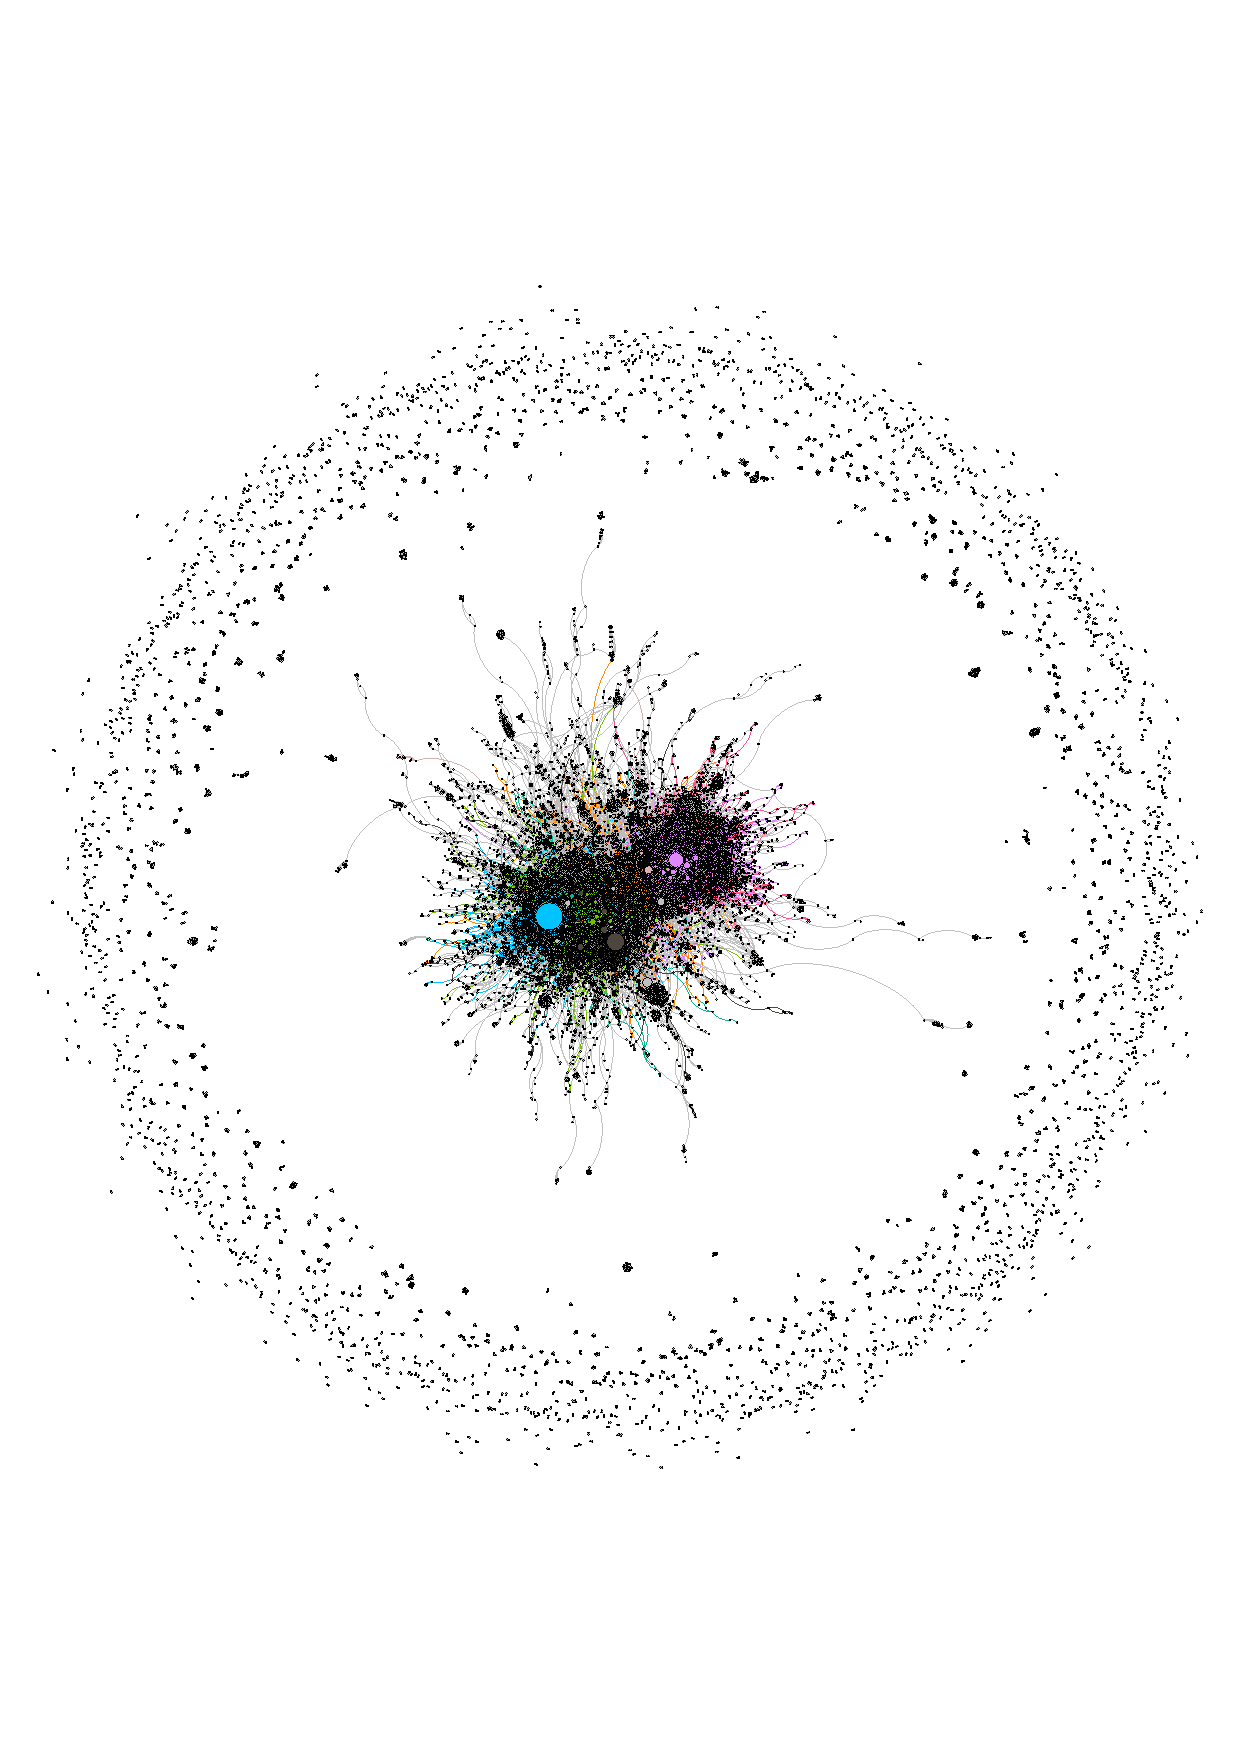
\includegraphics[width=\linewidth, height=\textheight, keepaspectratio]{img/net_hyperlocal_two.pdf}
        \end{subfigure}

        \begin{subfigure}{.45\linewidth}
          \caption{\se{Subset 3}\\ 6~May,~2013 -- 3~Mar.,~2016;\\ nodes: \num{29353}, edges: \num{22273}}
          \label{subfig:net_diac_hyperlocal_three}
          \centering
          % \includegraphics[width=\linewidth]{example-image-c}
          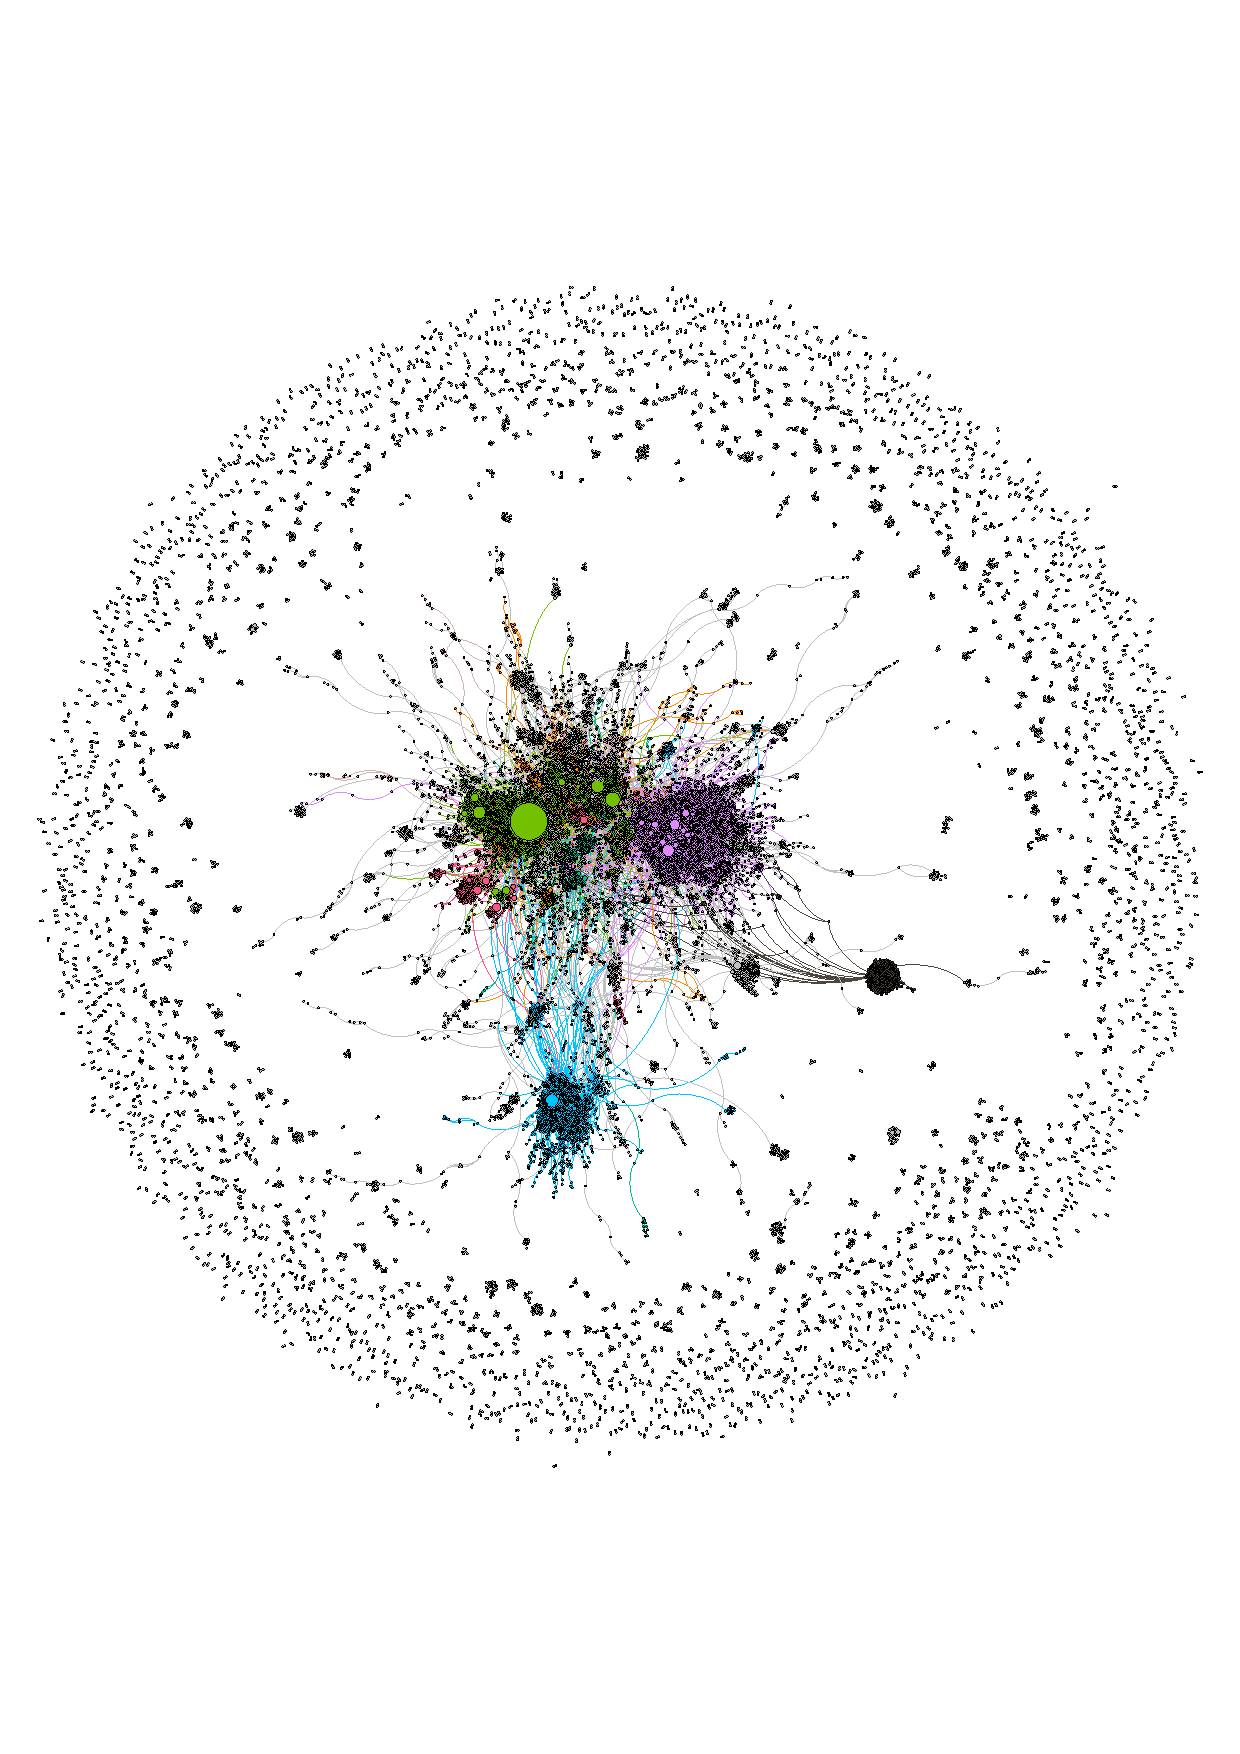
\includegraphics[width=\linewidth, height=\textheight, keepaspectratio]{img/net_hyperlocal_three.pdf}
        \end{subfigure}
        \begin{subfigure}{.45\linewidth}
          \caption{\se{Subset 4}\\ 4~Mar.,~2016 -- 31~Dec.,~2018;\\ nodes: \num{26548}, edges: \num{16576}}
          \label{subfig:net_diac_hyperlocal_four}
          \centering
          % \includegraphics[width=\linewidth]{example-image-a}
          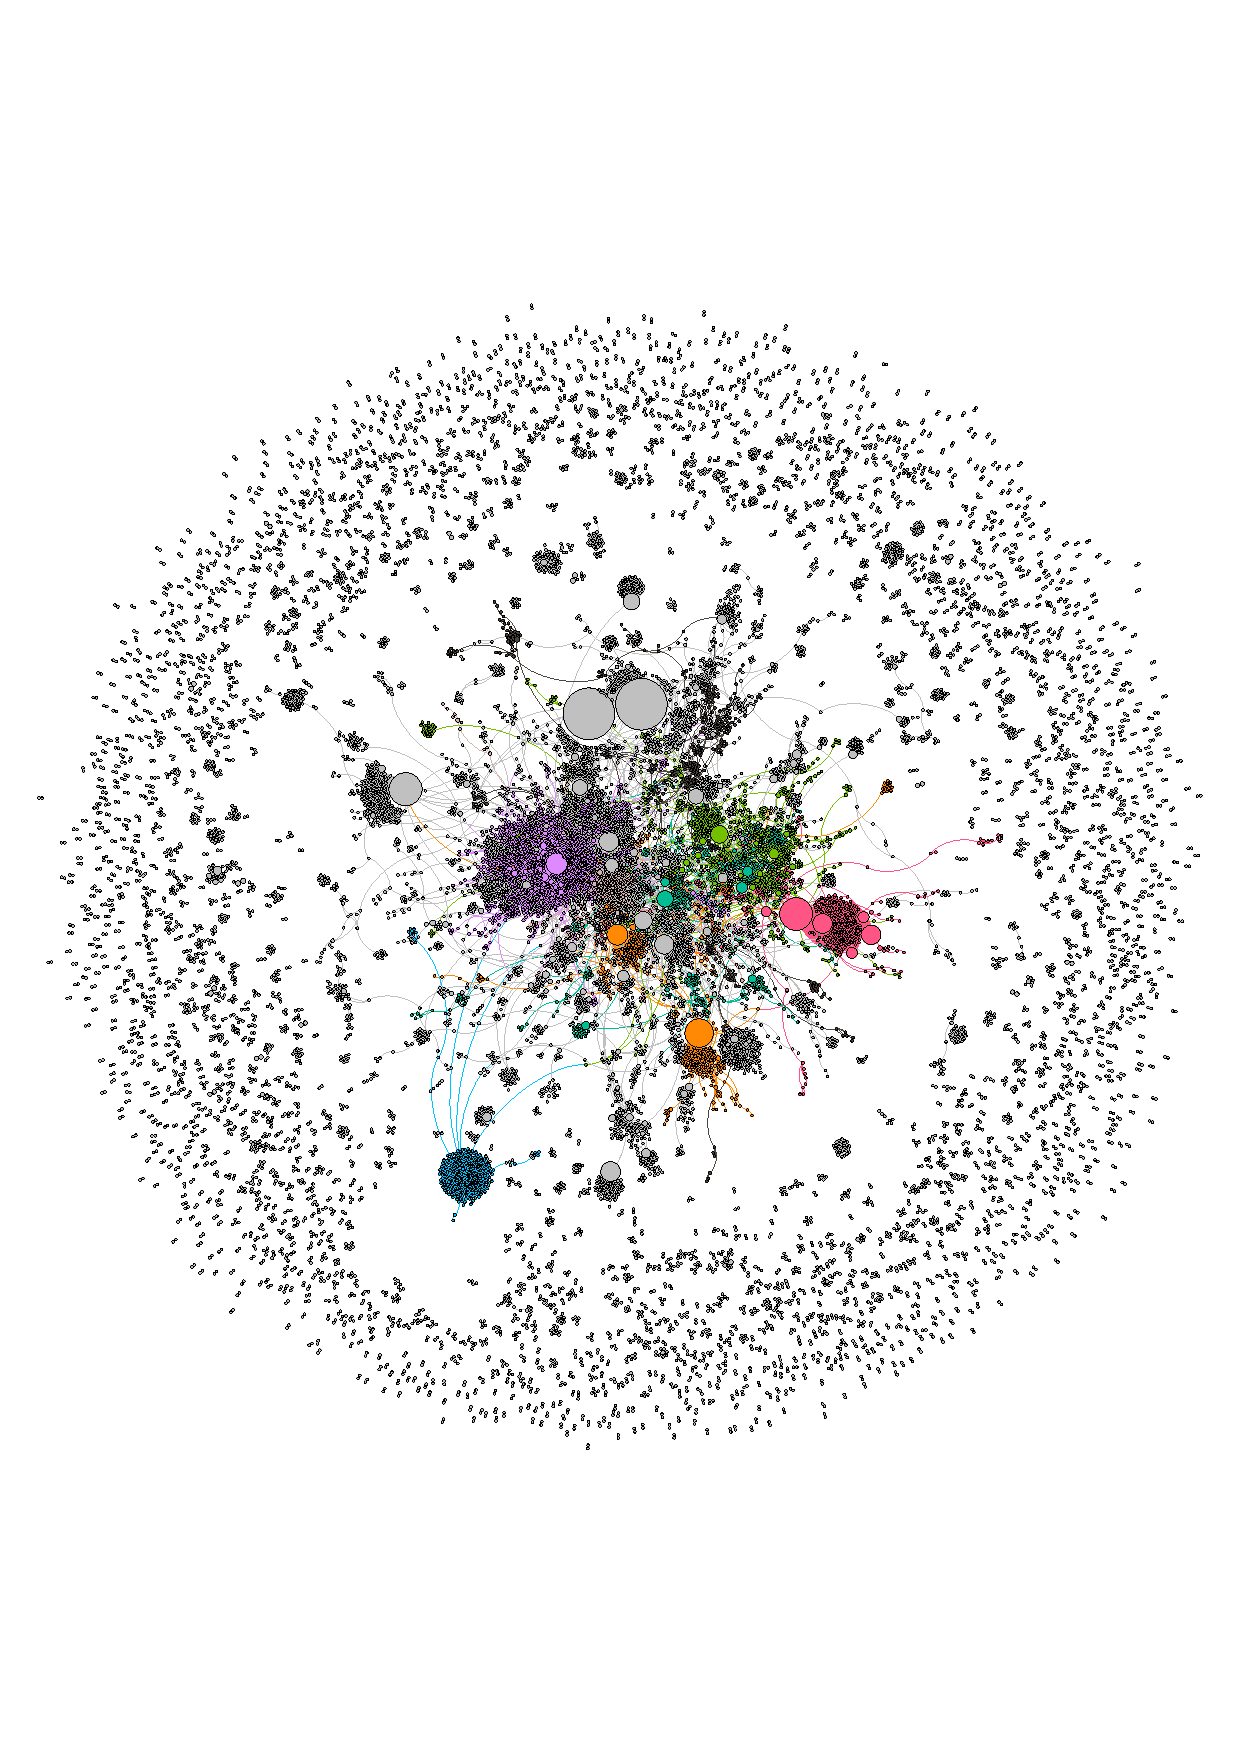
\includegraphics[width=\linewidth, height=\textheight, keepaspectratio]{img/net_hyperlocal_four.pdf}
        \end{subfigure}
        \caption[Social networks of diffusion for \ol{hyperlocal}]{Social network of diffusion for \ol{hyperlocal} over time.}
        \label{fig:net_diac_hyperlocal}
      \end{figure}

      Both the quantitative measure in Figure~\ref{fig:cent_diac_cases} and the network visualizations in Figure~\ref{fig:net_diac_hyperlocal} indicate that \ol{hyperlocal} shows increasing, successful diffusion over time.

      Its use is relatively centralized in its earlier stages, which can be seen from the fact that most speakers who have used the term are closely connected in the social graph in the first quarter of its observed lifespan. Inspecting the most influential speakers and sub-communities in the network (based on PageRank and Modularity scores) reveals that \ol{hyperlocal} is mainly used by a relatively small community of individual journalists in the first subset, who are early adopters in trying to target news to local audiences and use the term very frequently to label this new approach.

      In Subset 2, the community of journalists grows and starts to include also bigger news outlets such as The Guardian. Additionally, a new community of practice adopts the term: several marketing agencies start promoting their services using the term \ol{hyperlocal}. At this point, the usage intensity of the term peaks, as was demonstrated in Figure~\ref{subfig:freq_temp_hyperlocal}. However, the social network data indicate that at this point its use is still mainly the product of high salience and usualization within a small number of dense sub-communities rather than a sign of advanced diffusion across bigger parts of the speech community.

      The network graphs show that the social diffusion of \ol{hyperlocal} is only significantly advanced in the last two stages. While we see only few weak ties during the earlier stages of its use, the term now increasingly diffuses beyond its early adopters. Inspecting the network reveals that use of term becomes increasingly popular in the world of business and startups as well as the general public. The network metrics indicate that individual agents and sub-communities now play a far smaller role in its overall use. While \ol{hyperlocal} shows less usage intensity during these later stages, the network metrics indicate a high degree of diffusion for the second half of its observed lifespan. The timing of its addition to the OED in 2015 supports these observations. \ol{hyperlocal} has successfully spread beyond its subcommunities of early adopters, and it seems to be used by a diverse community of speakers from different backgrounds, which renders it a case of successful diffusion. This process of increasing diffusion for \ol{hyperlocal} is also reflected in its decreasing measures for graph centrality in Figure~\ref{fig:cent_diac_cases}.

      The remaining cases in Figure~\ref{fig:cent_diac_cases} show different pathways of diffusion, both in terms of their overall degree of diffusion as well as their diachronic trajectory. Due to space limitations, I can only provide an overview of their development over time.
      
      Besides \ol{hyperlocal}, the second neologism which exhibits advanced diffusion is \ol{upskill}.
      
      In this case, however, we observe little change over time, its degree centrality has been very low since its early attestations in the corpus. This suggests for an organic diffusion process which was not triggered or significantly shaped by the involvement of a small group of influential speakers alone. The term \ol{upskill} has been used by a wide variety of speakers throughout its observed lifespan and shows the highest degree of diffusion among the selected cases.

      By contrast, \ol{solopreneur} and \ol{poppygate} show a negative trend in terms of diffusion. The term \ol{solopreneur} features low degrees of diffusion in its earlier stages, but its use becomes more centralized over time. This is in contrast with its usage intensity over time (Figure~\ref{subfig:freq_temp_solopreneur}): while its earlier period of moderate use goes back to a decentralized community of users, its increase in usage frequency goes along with a narrowing of its user base. As the network analysis in Figure~\ref{subfig:net_last_cases_solopreneur} demonstrated, it becomes increasingly limited to a relatively small community which shares interest in a small professional niche.   

      The case of \ol{poppygate} exhibits a similar trend towards increasing centralization. Its temporal dynamics show a pattern or recurrent topical usage (Figure~\ref{subfig:freq_temp_poppygate}). The social networks of \ol{poppygate} suggest that while term was used by a broader audience in its earlier stages, its use in the more recent past goes back to certain communities of speakers for which a specific topical event emerges as a salient occasion to use the term. For example, its most recent spike in usage intensity in November 2016 was caused by a controversy about whether Fifa was right to take disciplinary action against the national teams of England and Scotland after their players wore poppy armbands during a football match between the two nations on 11 November. Protests by the football community caused a spike in usage intensity for \ol{poppygate}, but did not trigger its diffusion beyond this community.

      Lastly, \ol{alt-right} and \ol{alt-left} show limited degrees of diffusion over their lifespan. While the centrality of \ol{alt-right} remains fairly stable over time, \ol{alt-left} shows increasing centralization. Both terms are strongly tied to the political discourse surrounding the Unite the Right Rally in the United Stated and consequently exhibit a sharp increase in usage intensity in the course of the event in August 2017 (Figure~\ref{fig:freq-abs}). This increase in use is, however, reflected by increased centrality scores for both lexemes in Figure~\ref{fig:cent_diac_cases}. This period of highly intense use is thus characterised by relatively smaller rather than larger degrees of diffusion for both lexemes. While the use of \ol{alt-right} reverts to more decentralized use afterwards, the use of \ol{alt-left} remains at this high level of centrality. This seems to confirm the echo chamber effect for \ol{alt-left} discussed in Section~\ref{subsec:degrees-of-diffusion}: the term has become conventional and popular among a community of like-minded individuals, but its use remains limited to this community. Given the political orientations involved, it seems plausible that the majority of Twitter users do not want to be associated with this term nor its community of users.  

      In summary, studying the temporal dynamics of social networks highlights changes in the use of neologisms over time and reveals differenct pathways of diffusion in the sample.


  \subsection{Evaluating the frequency and network approaches}
    \label{subsec:nets-vs-freq}

    Having applied the frequency-based and the social network approach to assess the diffusion of the present sample of neologism, this section will evaluate and compare the results obtained from both approaches. Due to the prevalence of using frequency as an indicator of diffusion in previous work, I will largely use frequency as a base of comparison for evaluating the social network approach.\footnote{It should be noted that a strict evaluation of both approaches is in principle impossible without external data about the true degrees of diffusion for the neologisms under investigation. While such a gold standard for evaluation is inconceivable in the present context, it would be desirable to use additional data sources such as questionnaires, dictionaries or web corpus data for a more rigorous validation of the present approach. This will have to be left for future work.}

    \subsubsection{Correlations}

      A first evaluation of the social network approach to diffusion relies on the correlations of degree centrality with the total usage frequency of neologisms, with their volatility, and with their age as observed in the corpus. Table~\ref{tab:correlations} reports the correlation coefficients for these variables.

      \begin{table}
        \centering
        \caption[Correlation matrix for \textsc{centrality}]{Correlations of \enquote{degree centralization} (\textsc{centrality}) with the variables total usage frequency (\textsc{frequency}), coefficient of variation (\textsc{volatility}), and observed lifespan in the corpus (\textsc{age}) for the full sample of neologisms ($n=99$) using Spearman's correlation coefficient~\parencite{Spearman1961ProofMeasurement}.\protect\footnotemark{}}
        \label{tab:correlations}
        \begin{tabular}{>{\scshape}l r r}
          \toprule
                      & {$\rho$}    & P               \\
          \midrule
          frequency  & \num{-0.44} & $<$ \num{0.001} \\
          age        & \num{-0.29} & \num{0.004}     \\
          volatility & \num{0.28}  & $<$ \num{0.001} \\
          \bottomrule
        \end{tabular}
      \end{table}
      \footnotetext{All variables entering the correlation analysis were log-transformed and centred.}

      Firstly, centrality shows a significant negative correlation with \textsc{frequency}. This confirms earlier observations in Section~\ref{subsec:sna} which indicated an inverse trend between total usage frequency and centrality. More frequent neologisms show on average higher degrees of diffusion, i.e. their use goes back to less centralized communities of speakers. The fact these two central measures for diffusion correlate substantially can be seen as a cross-validation of both approaches. While external data sources would be needed for a more rigorous evaluation, this overall convergence in results suggests that both metrics capture important aspects of diffusion.

      Secondly, the \textsc{age} of neologisms in the sample shows a significant negative correlation with centrality. As expected, the use of more recent neologisms tends to still go back to more centralized communities, while neologisms with a longer history of use tend to show more advanced diffusion. Unlike frequency counts, which are directly influenced by the temporal usage history of neologisms, the centrality measure is blind to this information. The fact that these age effects are captured by degree centrality supports the validity of the social network approach.

      Lastly, \textsc{volatility} shows a significant positive correlation with centrality. Again, this result is in line with expectations. Neologisms such as \ol{poppygate}, whose use exhibits substantial temporal variation tend to show lower degrees of diffusion than neologisms such as \ol{hyperlocal}, whose use is more consistent and less dependent on the topical salience of extralinguistic events.

    \subsubsection{Deviations centrality between and frequency}

      For a closer analysis of the interactions between these variables beyond correlation coefficients, Figure~\ref{fig:cent-vs-freq} presents all neologisms according to their usage frequency and centrality scores. While Figure~\ref{subfig:cent-vs-freq_sample} covers the full sample, Figure~\ref{subfig:cent-vs-freq_cases} is based on the same data, but zooms in on the frequency range which covers four of the selected cases to provide a clearer view of this section of the graph.

      \begin{figure}
        \caption[Scatterplot of \textsc{usage frequency} and \textsc{centrality}]{Relationship between total \textsc{usage frequency} and degree centrality (\textsc{centralization}) for the full sample of neologisms ($n=99$) and the selected cases.}
        \label{fig:cent-vs-freq}
        \centering
        \begin{subfigure}{.49\linewidth}
          \caption{Full sample.}
          \label{subfig:cent-vs-freq_sample}
          \centering
          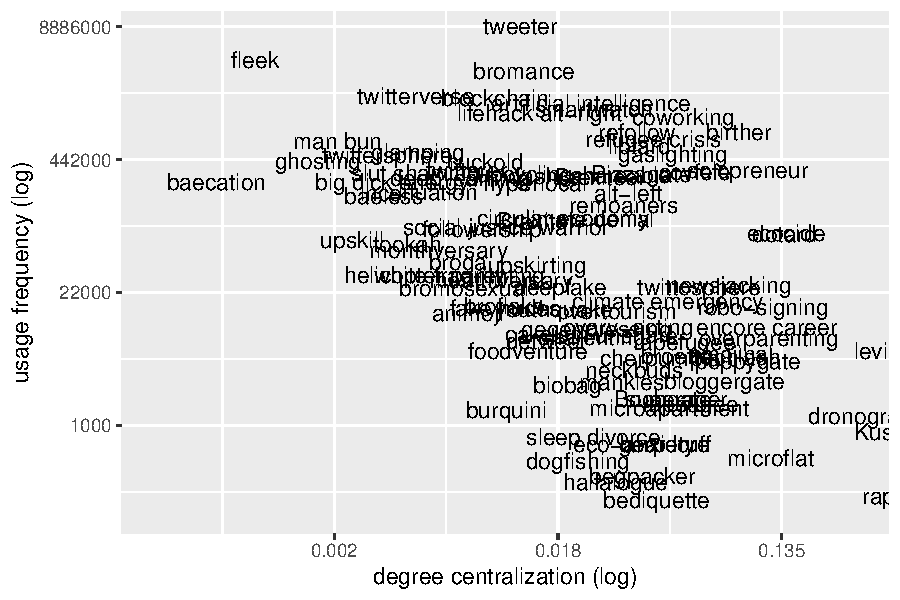
\includegraphics[width=\linewidth, height=.8\textheight, keepaspectratio]{img/full_cent_freq_overall.pdf}
        \end{subfigure}
        \begin{subfigure}{.49\linewidth}
          \caption{Selected cases.}
          \label{subfig:cent-vs-freq_cases}
          \centering
          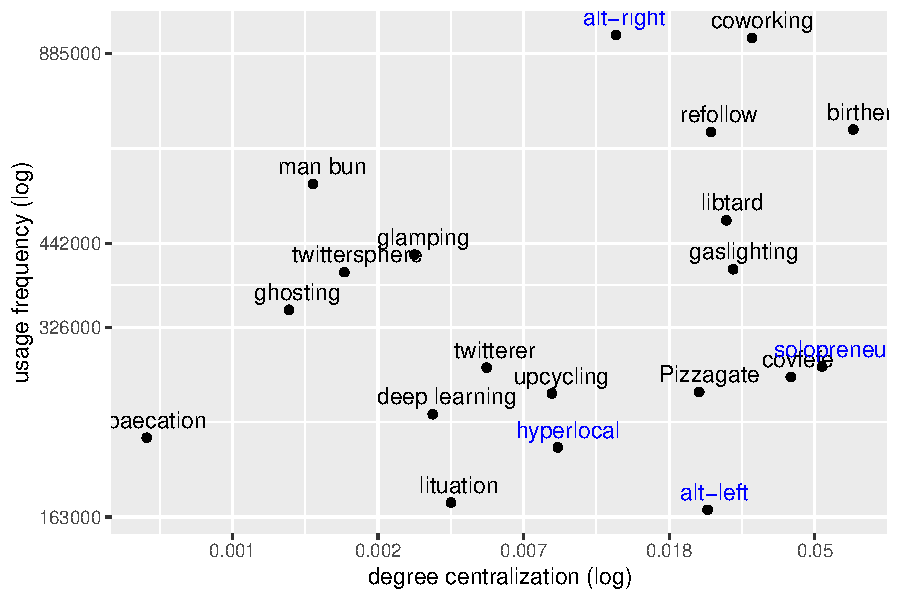
\includegraphics[width=\linewidth, height=.8\textheight, keepaspectratio]{img/cases_cent_freq_overall.pdf}
        \end{subfigure}
      \end{figure}

      The general trend in the plot confirms the inverse relation captured by the negative correlation coefficient between centrality and frequency. Neologisms with high frequency such as \ol{fleek} have low centrality scores and would thus be assigned a high degree of diffusion by both approaches. The inverse applies to candidates from the lower end of the frequency spectrum such as \ol{microflat}.

      However, Figure~\ref{subfig:cent-vs-freq_sample} also shows substantial variation between frequency and centality scores. Notably, the observed deviations are almost exclusively found towards the right of the diagonal trend, i.e. for cases where centrality assumes lower degrees of diffusion than frequency. For examples, while \ol{fleek} and \ol{bromance} are assigned similar scores in terms of their usage frequency, their centrality scores suggest a much lower degree of diffusion for the latter neologism. Similar to cases like \ol{solopreneur} and \ol{alt-left}, which were discussed in detail in Section~\ref{subsec:degrees-of-diffusion}, centrality thus seems to provide diverging results for cases in which the social network structure suggests that the observed usage intensity overestimates the degree of diffusion of a target neologism since its observed uses go back to a disproportionally smaller number of speakers and subcommunities.

      Analysing these deviations highlights at two main groups of neologisms, for which total usage frequency and social network structure seem to diverge in systematic ways. A first group contains neologisms which show high degrees of volatility in their frequency of use. As shown above, centrality is significantly correlated with volatility. In addition to \ol{poppygate} and \ol{solopreneur}, which were already discussed above, \ol{refollow}, \ol{gaslighting}, \ol{solopreneur}, and \ol{coworking} also show little consistency in their usage. For all of these terms, centrality assumes lower degrees of diffusion than total usage frequency counts in Figure~\ref{subfig:cent-vs-freq_sample}. It thus seems that the social network approach provides a more accurate picture in cases where frequency-based measures overestimate degrees of diffusion due to the strong impact of short periods of highly intensive use of neologisms in certain parts of the speech community.

      A second group with diverging scores contains neologisms whose use is tied to political communities. The neologisms \ol{alt-right}, \ol{alt-left}, \ol{birther}, \ol{covfefe}, \ol{Pizzagate}, and \ol{Kushnergate} are politically controversial and differ strongly in popularity between political camps. It should be noted that these terms also exhibit considerable volatility in their use. Figure~\ref{subfig:cent-vs-freq_sample} shows comparatively lower centrality than frequency scores for these lexemes. Similarly to the cases of high volatility, centrality thus suggests that usage frequency overestimates degrees of diffusion for these cases. While neologisms such as \ol{alt-right} show high frequency counts, the social network analysis reveals that these terms have not spread successfully across communities, and that their use remains limited to certain subcommunities.

    \subsubsection{Predicting the success of lexical innovations}

      The evaluation of the network approach shows that community structure can be used to assess degrees of diffusion. The social structure of communities during the early stages of diffusion is commonly assumed to be an important factor for the successful spread of linguistic innovations. While a detailed analysis is beyond the scope of the present paper, the present approach yields initial results of the predictive power of social network information.

      The dataset shows a significant correlation between the network structure in the first period of diffusion and the overall success of neologisms. Correlating \textsc{centrality} scores for all neologisms in Subset 1 with their total usage \textsc{frequency} observed across their full observed lifespan in the corpus yields Spearman correlation coefficient of \num{-0.43} (${P < 0.001}$). This means that neologisms are overall more likely to spread successfully if their use is not limited to a centralized network of speakers in their early stages. Among the selected cases presented above, \ol{upskill} fits this pattern: it shows a consistent, successful trajectory of diffusion and its use has been the product of a decentralized community of users since its early attestations. Of course, the diverging pathways of diffusion for other words such as \ol{hyperlocal} and \ol{solopreneur} presented in Figure~\ref{fig:cent_diac_cases} represent exceptions to this general trend. While this trend fits theoretical expectations and the empirical observations in the present dataset, these present results are only preliminary. Since centrality correlates with frequency scores, future work based on bigger samples, external data for evaluation, and more robust statistical tests is needed to test whether the predictive power of social network features can be confirmed.

\section{Discussion}
  \label{sec:discussion}

  In this paper, I have studied the spread of neologisms on Twitter to analyse degrees and pathways of diffusion of lexical innovations. The process of diffusion is fundamentally tied to social processes which involve the spread of innovations in social networks~\parencite{Rogers1962DiffusionInnovations}. According to most theoretical models, successful diffusion of linguistic innovations crucially involves their spread to new speakers and communities~\parencite{Weinreich1968EmpiricalFoundation,Schmid2020DynamicsLinguistic}. Despite broad consensus over the fact that diffusion entails spread in networks of speakers, most previous work has not been able to conduct large-scale empirical investigations on the basis of social network information. Lacking the necessary data and methods for studying diffusion in social networks directly, most previous studies have had to rely on using the frequency of occurrence of linguistic innovations as an approximate indicator of diffusion~\parencite{Stefanowitsch2017CorpusbasedPerspective}.

  The present study used data from Twitter to compile a large dataset which allowed to investigate the sociolinguistic dynamics of diffusion of neologisms in online social networks. Aside from an in-depth analysis of the diffusion of neologisms in the present sample, the aim of this paper was to assess the validity of using usage frequency and social network data as indicators of diffusion. While the results of this evaluation are most relevant to the study of \emph{lexical} \emph{innovations}, as I will argue, the findings also have general implications for corpus-based studies which rely on frequency or network measures to assess the conventionality of linguistic constructions.

  \subsection{Frequency}

    The frequency-based analysis revealed that several usage frequency based measures can be used to assess degrees of diffusion of lexical innovations with varying success.

    Total frequency counts (Table~\ref{tab:freq-total}) proved successful for a coarse-grained distinction between cases of high (e.g. \ol{tweeter}, \ol{smartwatch}), medium (e.g. \ol{monthiversary}, \ol{helicopter parenting}) and low degrees of diffusion (e.g. \ol{begpacker}, \ol{bediquette}).

    However, differences in the temporal dynamics of use turned out to be crucial for a more accurate assessment of degrees and pathways of diffusion of neologisms.

    Considering the nature of the process and products of \emph{lexical} innovation, this temporal sensitivity seems unsurprising. Typically, models of linguistic diffusion such as the S-curve model assume competition processes between several formal variants, in which they compete to become the conventional linguistic means to express a certain meaning/function in the speech community. In cases of grammatical innovation, which is at the core of most models and previous empirical investigations of diffusion, the communicative need for expressing the target concept/function remains stable over time. While the grammatical means in a language might change (e.g. \ol{going to}, \ol{will}), the salience of the target semasiological space (e.g. \mn{expressing future intention}) remains stable for all speakers in the speech community. Both competition between variants and the social and temporal invariance of the conceptual space over time are prerequisites to the S-curve model of diffusion \parencite{Blythe2012ScurvesMechanisms}

    Previous work by \cite{Nini2017ApplicationGrowth} has suggested that the diffusion of lexical innovations also follows S-curve trajectories and uses the term \enquote{semantic carrying capacity} to refer to the functional potential of neologisms during diffusion. However, it remains unclear whether the semantic carrying capacity of neologisms can be considered temporally and socially invariant, and whether, due to the open nature of the lexicon, competition effects between neologisms match the zero-sum competition between grammatical variants.

    Firstly, trends in usage frequency provide information about changes in diffusion over time.

    trend
    age
    volatility

  \subsection{SNA}

    diffusion
      number of speakers
      number of communities

    corpus-as-input, corpus-as-output \parencite{Stefanowitsch2017CorpusbasedPerspective}

    particularly important for \emph{lexical} \emph{innovations} due to the nature of the process
        bound to cultural conceptual salience (variable \enquote{semantic carrying capacity}~\parencite{Nini2017ApplicationGrowth})
        strong social indexicality
        coined consciously within tight-knit communities (c.f. grammatical innovation)

    case studies
      equally frequent words show different
        degrees of diffusion
        pathways of diffusion

    S-curve model
      role of early adopters / network structure
      influencers
      weak ties

    discrepancies
      volatile
      echo chambers

    better extrapolate beyond current dataset than frequency (e.g. web)


    also attractive for other linguistic domains
      potential for (computational) sociolinguistics, sociolinguists should \enquote{upskill}
      extend sociolinguistic research (on geographical variation; desideratum in \cite{Grieve2019MappingLexical})


  \subsection{Future work}

    \begin{qitem}
      # cross-validation of frequency and SNA information with other data sources
        ## systematic comparison with web data, e.g. NOW corpus~\parencite{Davies2013CorpusNews}; early attempts:~\cite{Wurschinger2016UsingWeb}
        ## questionnaires; early work:~\cite{Kerremans2015WebNew}
        ## dictionaries (e.g. Urban Dictionary)
      # investigate on diffusion across
        # contexts: different web registers~\parencite{Biber2016RegisterVariation}
        # cotexts: study differences in use between communities
          ## semantic innovation, meaning change
          ## variation and change between communities: \cite{Tredici2019YouShall}, \cite{Schmid2020BattlingSemantica}
      # predict the success of lexical innovations
    \end{qitem}

\section{Conclusion}
  \label{sec:conclusion}

%section{Bibliography}

  \printbibliography

% \section*{Acknowledgements}

%   \begin{itemize}
%     \item UI: Max, Fabi
%     \item SNA: Kauermann group
%     \item Hans-Jörg
%   \end{itemize}

\end{document}
